\documentclass[a4paper,11pt,titlepage]{article}
\parskip 3pt

%% %%%%%%%%%%%%%%%%%%%% BEGIN PACKAGES %%%%%%%%%%%%%%%%%%%%

%%\usepackage[top=1in, bottom=1in, left=1in, right=1in]{geometry}

%%\usepackage{fullpage}
\usepackage{url}
\usepackage{hyperref}
\usepackage{listings}
\hypersetup{pdfborder=0 0 0}

%% Images
\usepackage{graphicx}

%% Side-by-side images
\usepackage{subfig}

%% Wrapped figures
\usepackage{wrapfig}

%% Drawing trees and other stuff
\usepackage{tikz}
\usetikzlibrary{trees,arrows}
\usepackage{amssymb}

%% Pseudocode
\usepackage[noend]{algorithmic}
\algsetup{indent=1.5em}

%% Linux Libertine
\usepackage[T1]{fontenc}
\usepackage{libertine}
\renewcommand*\oldstylenums[1]{{\fontfamily{fxlj}\selectfont #1}}

\definecolor{cffffff}{RGB}{255,255,255}
\definecolor{c787aff}{RGB}{120,122,255}
\definecolor{cff7374}{RGB}{255,115,116}
\definecolor{c79ff79}{RGB}{121,255,121}
\definecolor{cff7374}{RGB}{255,115,116}
\definecolor{c7372ff}{RGB}{115,114,255}
\definecolor{c63ff63}{RGB}{99,255,99}
\definecolor{c6365ff}{RGB}{99,101,255}
\definecolor{darkgreen}{RGB}{0,162,0}
\definecolor{darkred}{RGB}{162,0,0}


\let\stdhref\href
\renewcommand{\href}[2]{\stdhref{#1}{\texttt{#2}}}

\newcommand{\mailto}[1]{\href{mailto:#1}{#1}}

\let\stdsection\section         % because LaTeX cannot handle
                                % recursive commands
\renewcommand{\section}{\newpage\stdsection}

\let\tikzsquare\square
\renewcommand{\square}{\ensuremath\tikzsquare}

\newcommand{\code}[1]{\texttt{#1}}
\newcommand{\buzz}[1]{\emph{#1}}
\newcommand{\magic}[1]{\buzz{#1}}

\newcommand{\myhref}[1]{\href{http://#1}{#1}}

%% Acronyms, names, blah
\newcommand{\Qt}{\buzz{Qt} }
\newcommand{\OpenGL}{\buzz{OpenGL} }
\newcommand{\FADE}{\buzz{FADE} }
\newcommand{\master}{\code{master} }
\newcommand{\Git}{\buzz{Git} }
\newcommand{\Cairo}{\buzz{Cairo} }
\newcommand{\Twitter}{\href{http://twitter.com}{Twitter} }
\newcommand{\GitHub}{\href{https://github.com}{GitHub} }

%% Clubs and widows. Avoid them like the plague.
\clubpenalty = 10000
\widowpenalty = 10000
\displaywidowpenalty = 10000

%% %%%%%%%%%%%%%%%%%%%% END COMMANDS %%%%%%%%%%%%%%%%%%%%

%% %%%%%%%%%%%%%%%%%%%% BEGIN COLORS %%%%%%%%%%%%%%%%%%%%


%% %%%%%%%%%%%%%%%%%%%% END COLORS %%%%%%%%%%%%%%%%%%%%


%% Final Report -- due: 9th Jan 2012, at 11:00
%% Contents for Final Report: The project report should not be longer than 45
%% pages, and might be organized according to the following structure:

%% A. High Level, Nontechnical Description Why you should buy this
%% product/listen to this presentation? What is the functionality of the
%% product?

%% B. Short Technical Description
%% Short introduction into technologies used Design of your software, possibly
%% including a diagram of the major components of the project Main achievements

%% C. Software Engineering Issues:
%% What technology was used and why; what other technology was considered but
%% not used and why
%% Any technical challenges encountered and how addressed
%% Any risks anticipated, and how mitigated?
%% Any collaboration/coordination difficulties encountered and how addressed
%% Development and testing methods and/or tools used; comparison of plans with
%% actual achievements
%% Estimates of length of code in each of the components, or any other
%% comparable measure of the effort required.
%% Summary of each team member's contributions

%% D. Validation and Conclusions How did you validate your product? Was the
%% project successful? What did you learn? What might you have done differently?

%% E. Bibliography

%% F. Appendix The appendix is optional, and does not count towards the 45
%% pages. It may contain thing like: User guide, installation instructions; more
%% extensive design, testing, statistics etc.

%% Feel free to re-use material from the previous reports as you see fit, but
%% make sure that the final report presents a coherent story. Ask advice from
%% your supervisor. You might also draw inspiration from the instructions about
%% writing up your individual project.
%% Bear in mind, that most of the project assessors will not have followed the
%% project throughout and will only have a short time to listen to a
%% presentation or see a demonstration. For this reason they will rely heavily
%% on the report to judge the project.
%% The report should be submitted to SGO in form of a hard copy, as well as
%% electronically through CATE.

\begin{document}
\title{
\includegraphics[width=2cm]{v.png}\\
  \Huge Visigoth\\\Large Graph visualisations}
\author{
  Andreea-Ingrid Funie\\\mailto{aif109@doc.ic.ac.uk}\and
  Alexandru Scvor\c tov\\\mailto{as10109@doc.ic.ac.uk}\and
  Francesco Mazzoli\\\mailto{fm2209@doc.ic.ac.uk}\and
  Marc-David Haubenstock\\\mailto{mh808@doc.ic.ac.uk}\and
  Maximilian Staudt\\\mailto{ms9109@doc.ic.ac.uk}
}
\date{January 2012}
\maketitle

\begin{abstract}
Visigoth is a tool to generate, analyse and visualise Small World
Networks. These are particular kinds of graphs which \emph{look} like naturally
grown networks and share many mathematical properties with them.  For instance,
friendship graphs and graphs of followers in modern web-based ``social
networks'' are Small World Networks.

As an educational tool Visigoth allows users to explore Small World Networks and
hence can be used as an introduction to them. By exploring these networks users
will have a firmer, more intuitive grasp of the mathematical properties they
exhibit.

The networks may be generated using several algorithms, allowing users to
compare their output and its adherence to the properties of Small World
Networks. The network generation algorithms in Visigoth form a smooth
progression in the number of exhibited desired properties from completely random
graphs, generated by the Erd\H{o}s-R\'{e}nyi algorithm, to fully compliant Small
World Networks, generated by the Preferential Attachment
algorithm. Additionally, Visigoth can connect to social networking platforms
such as \Twitter to fetch and display real-world networks.
\end{abstract}



\tableofcontents



\section{Introduction}
%% This section corresponds to A in the requirements.

%% This section should contain most of the references to hamm10 and
%% oconn11.

Complex networks are ubiquitous in nature and society.

The dynamics and structural properties of complex networks are non-trivial,
making performant computation gear a requirement for their statistical
analysis. As such it has only become feasible to study real networks with their
large underlying data sets within the last decade.  \cite{oconn11}

The structural properties of real networks have been studied extensively over
the years, mainly focusing their common characteristic properties.  These
networks share low average distances, high clustering coefficients and
scale-free degree distribution.

In order to easen further analysis of real networks, the aim is to simulate them
using procedurally generated networks. However, this requires the generation
algorithms used to output networks which are true to the characteristic
structural properties of \emph{Small World Networks}.

\subsection{Realistically looking networks}
%% This subsection should *not* use the term ``Small World Networks''.
%% The point is to describe what properties we want.  The SWN
%% subsection below should be used in order to explain how they fit
%% the requirements.

%% FIXME: Define the qualities of the networks we want.  These
%% shouldn't be too mathy, just a layperson explanation (e.g. the
%% nodes shouldn't be too far apart, the number of neighbours should
%% fit a natural distribution).

The networks of interest here are mathematical graphs in which most nodes, while
not being connected directly, can be reached from any other node via a small
number of steps. In the context of a social network this results in the ``small
world phenomenon'' \cite{swphen} of strangers being linked by a mutual
acquaintance.

Social networks, neural networks, the World Wide Web, electrical power grids and
protein structures are all examples for complex networks the precise dynamic
behaviour of which currently escapes our understanding.

\begin{figure}[ht!]
  \centering
  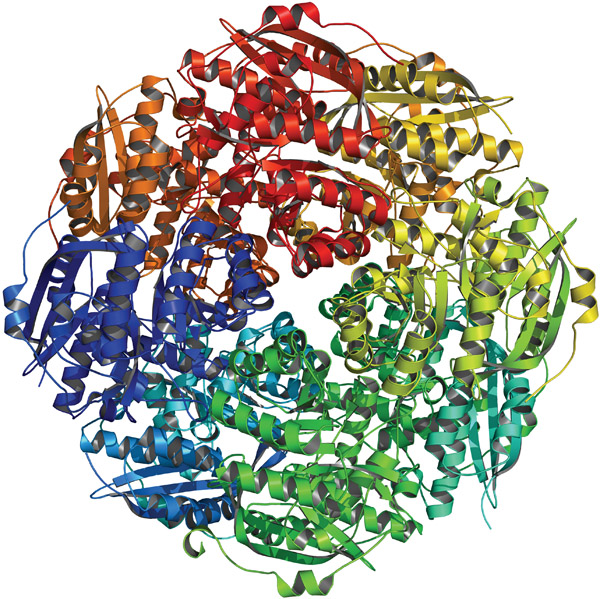
\includegraphics[height=50mm,width=50mm]{protein-structure.png}
  \caption{Protein structure}
  \label{fig:protein}
\end{figure}

% FIXME: Maybe we can add here a picture of some neural networks in the brain?

Results from network science have been applied to the analysis of metabolic and
genetic regulatory networks, the design of robust and scalable communication
networks, the development of vaccination strategies
for disease control and a broad range of other practical
uses. \cite{complexNets}


\subsection{The maths}

%% FIXME: Give formal mathematical definitions for qualities.

\subsubsection{Networks}

A \emph{network} is, in the mathematical sense, a graph. This
graph in turn consists of a set $N$ of \emph{nodes} and a set
$E$ of \emph{edges}. An edge is a connection between two nodes
and can be mathematically represented as a pair thereof.


\subsubsection{Degree of a node}

The \emph{degree} $k_i$ of a node $n_i$ is the number of nodes that it is
connected to. The average degree $K_{avg}$ of a network is
\[ K_{avg} =\frac{2 \cdot |E|}{|N|} \]
where $|E|$ is the number of edges in the network and $|N|$ is the total
number of nodes. The factor of $2$ takes into account that every edge is
connected to two nodes.

\subsubsection{The small world effect}

The concept of ``six degrees of separation'' is the idea that if the
acquaintances between all human beings on Earth were to be recorded
in a graph, everyone would be at most approximately six hops (from
acquaintance to acquaintance) away from any other person on Earth.

In such a graph, a sequence of edges from one individual to another is
called a \emph{path}, and the length of the \emph{shortest} possible path
(also called the \emph{distance}) is of special interest as it tends to
be surprisingly low in natural networks, even if they consist of as many
as billions of nodes - such as the human population.

Frigyes Karinthy first introduced the idea of ``six degrees of separation''
in his 1929 short story ``Chains''.

Later on the small world experiment, performed in the 1960s by
Stanley Milgram and other researchers, formalised the
aforementioned concept. In this experiment letters were
sent to random individuals, asking them to forward the letter to a
random recipient. In case the destination was unknown to them
they were instructed to send the letter to a friend or
relative who was more likely to know the recipient.
The conclusion Milgram drew from his experiment was that the
distance between any two individuals is on average $6$.

This result led to the more genereal idea of a ``small world effect'' which
describes the idea that the average distance linking two nodes belonging to
the same network can be orders of magnitude smaller than the number of nodes
the network actually consists of. \cite{complexAdapt}

The characteristic properties of a small world network are:

\begin{itemize}
  \item Low average distance.
  \item High clustering coefficient.
  \item Scale-free degree distribution.
\end{itemize}

These characteristics shall be explained in more detail in the following subsections.

\subsubsection{Distance}

As mentioned before, the \emph{distance} between two nodes in a graph
is the minimum number of edges to be traversed in order to get from
the first node to the second.

Both Dijkstra's algorithm and A* can be used to find the distance
$d(n_i, n_j)$ between two nodes $n_i$ and $n_j$ in a network. The
average distance $d_{avg}$ in a network of $|N|$ nodes is the average
of the distance over all pairs of nodes:

\[ d_{avg} = \frac{1}{|N| \cdot (|N| - 1)} \sum_{i, j} d(n_i, n_j) \]

where $d(n_i, n_j) = 0$ when there is no path from $n_i$ to $n_j$.

\subsubsection{Clustering coefficient}
\label{sec:clusteringcoefficient}

\emph{Clustering} is the tendency of real networks to form
\emph{cliques}. In a graph, a clique is defined to be a subset of
nodes in which all nodes are connected to each other.
In real life, cliques represent circles of friends
or acquaintances in which every member knows every other member.

The clustering coefficient $C_i$ of a node $n_i$ as proposed by
Watts and Strogatz is defined as

\[ C_i = \frac{2 \cdot |E_i|}{k_i \cdot (k_i-1)} \]

where $k_i$ is the number of neighbours of node $n_i$ and $|E_i|$ is
the number of edges between the neighbours of node $n_i$. Thus, the
average clustering coefficient $C_{avg}$ over a network of $|N|$
nodes is:

\[ C_{avg} = \frac{1}{N}\sum_{i=0}^{N} C_i \]

\subsubsection{Scale-free distribution}
\label{sec:scale-free}

Barabasi and Albert showed that real networks such as the World Wide Web
are \emph{scale-free}. In these networks, the \emph{degree distribution}
follows the power law

\[ P(k) \sim k^{-\gamma} \]

where $P(k)$ is the probability that a node will be of degree $k$.


\subsection{Small world networks}

Small-world networks tend to contain \emph{cliques} and
\emph{near-cliques}, meaning sub-networks which have connections
between almost any two nodes within them. This stems directly from
the defining property of having a high clustering coefficient.

Secondly, most pairs of nodes will be connected by at least one
\emph{short path}, i.e. a path that is shorter than the
\emph{average distance}.
This follows from the property that the average distance $d_{avg}$
is small even when the total number $|N|$ of nodes is large.

Several other properties are often associated with small world
networks. Typically there is an over-abundance of hubs - nodes
in the network with a high number of connections (called a high
degree of the respective node). These hubs serve as the common
connections mediating the short distances between other
nodes. By analogy, the small-world network of airline flights
has a small average distance, i.e. between any two cities one
is likely to have to take three or fewer flights because many
flights are routed through hub cities. \cite{smnet}

Small world properties are found in \emph{many} real-world
phenomena including road maps, food chains, electric power
grids, metabolic processing networks, networks of brain
neurons, voter networks, telephone call graphs, and social
influence networks.

Networks of \emph{connected proteins} have small world properties
such as power law obeying degree distributions. Similarly,
\emph{transcriptional networks} with genes as the nodes,
linked if one gene has an up- or down-regulatory genetic
influence on the other, have small world network properties.

%% FIXME: Explain how SWNs exhibit *all* the properties we're
%% interested in.  Include some math.


\subsection{Introducing Visigoth}

Visigoth makes peeking into the current state-of-the-art of artificial Small
World Networks simple and fun. By integrating existing generation algorithms and
visualisations into a single, easy-to-use interface, the user can make a head
start into the large world of small world networks and

\begin{itemize}
  \item see how these algorithms have improved on each other over time,
    generating increasingly better networks,
  \item see the effects of changing algorithm parameters on the
    resulting networks, and
  \item compare them to naturally grown networks.
\end{itemize}

\subsection{Customer requirements and iterative (re-)specification}

% What our customer wanted.
%
% What we suggested, and what he finally wanted.
% (E.g. once we suggested 3D he didn't want to let go of the idea)
%
% Finally, on overview of what we did, and what we added as a bonus.
% Possibly another subsection.

Our customer initially asked for a simple, easy-to-use, graphical
application that would allow him to compare various Small World
Network generation algorithms and parameters thereof, both visually
by looking at the graphs as well as numerically by calculating
several statistical properties of the graphs.
We suggested several additional features, such as a 3D view of the
graphs generated, real-world data fetching from social networks
(\Twitter) and graph interaction. Following our customer's highly
positive reaction to our suggestions we then added them to our
product, creating a comprehensive base for analysing graphs that
may be re-used for other mathematical projects in the future.

\section{Visigoth functionality}

% FIXME: Describe what we can do. Generate, set properties, save
%        screenshots, move nodes, fly in 3D, the kitchen sink.

\subsection{Graph display}
Visigoth is able to draw graphs in both 2D and 3D, showing the graph
either in a planar display or in ``space'' and thus allowing the user
to ``fly'' through it. Notably, the user can switch between the two
modes at any time while preserving the graph.

\subsection{Graph Generation}
Visigoth uses the 5 algorithms described in section \ref{sec:algos} to generate
graphs for the user to interact with:

\begin{description}
\item [Preferential Attachment with Clustering] Selects a node for attachment
  depending on the number of edges they hold compared with the whole
  system. Creates links to nodes neighbouring that node.

\item [Bipartite Generation] Creates a bipartite graph and for all nodes, links
  all nodes of set A connected to the same node in set B. Finally, removes all
  nodes form set B.

\item [Erd\H{o}s-R\'{e}nyi] Generates a random graph.

\item [Watts-Strogatz] Creates a ring of connected nodes and re-links some nodes
  randomly within that ring.

\item [Barab\'{a}si-Albert] Nodes added to by preferential attachment, with no
  clustering.
\end{description}

In addition to these algorithms, we also implement a \Twitter data-mining
option, which lets users use their \Twitter account to graph the relations
between followers starting from themselves.

The algorithms may be configured by a variety of parameters exposed to users
via inputs. Most algorithms may also be later expanded by adding nodes.

\subsection{Graph Interaction}
There are several ways to interact with the graph: by \emph{dragging} it using
the mouse, the graph is moved on the screen. In 3D mode, it can also be rotated
and moved back and forth.

Similarly, nodes can be dragged using the mouse, resulting in a reordering of
the graph according to the built-in spring force model. \emph{Clicking} a node
calculates node specific statistics, such as the clustering coefficient.

A \emph{toolbar} gives easy access to common actions such as graph regeneration
and node reshuffling.

A simple \emph{menu} option allows users to customize the appearance of the
generated graph, such as: change edges and nodes colour, choose a different
background, highlight cliques or highlight selected node and connections with
it's direct neighbours.

\subsection{Export to PNG, JPEG files}
Finally, Visigoth allows taking snapshots of the graphs and exporting them to
image files. The supported formats include PNG and JPEG, which are the image
formats supported by most computers.

\section{Generating Small World Networks}
\label{sec:algos}
%% For all of the following, we should include a hand-drawn sketch
%% illustrating the graph generated by the algorithm and an exported
%% image of a large graph Visigoth generated.

On request of our customer we have implemented several generation
algorithms for Small World Networks which have been developed over
the course of the last decade.


\subsection{Erd\H{o}s-R\'{e}nyi}
The Erd\H{o}s-R\'{e}nyi model, named after Paul Erd\"{o}s and
Alfr\'{e}d R\'{e}nyi, is an algorithm to generate random networks.
This is the simplest of the graph generation algorithms in Visigoth's
repertoire, but while this makes it quite attractive,
the random networks produced by this model do not exhibit all of
the characteristics of real networks since clustering is low and
the node degree distribution is binomial (and thus not scale-free).

Edges in the network are created depending on a probability cutoff
value which can be set by the user. For every pair of nodes in the
network, a new random number is generated and the nodes are linked
by an edge if the random number is below the cutoff value.

In the following pseudocode for this algorithm, $N$ is the number
of nodes in the graph, while $P$ is the probability cutoff value:

\begin{algorithmic}
  \REQUIRE $0 \leq P \leq 1$
  \FOR{$i = 0 \to N - 1$}
    \FOR{$j = i + 1 \to N - 1$}
      \STATE $k \gets $ random real in $[0, 1]$
      \IF{$k < P$}
        \STATE Add edge between $i$ and $j$.
      \ELSE
        \STATE \textbf{continue}
      \ENDIF
    \ENDFOR
  \ENDFOR
\end{algorithmic}


\subsection{Watts-Strogatz}
The Watts-Strogatz model is a graph generation algorithm which
generates random graphs with the small world properties of
\emph{low average distance} and \emph{high clustering}.
It was invented by Duncan J. Watts and Steven Strogatz in 1998.

This model is based on stochastically `rewiring' the edges of a
regular ring lattice. The resulting network is a trade-off
between a regular ring lattice and a random Erd\H{o}s-R\'{e}nyi
network, therefore giving a great variation of possible output
networks depending on the probabilities for both the initial
connection of nodes as well as the rewiring of edges.

The algorithm operates in two steps:

\begin{itemize}
  \item First, generate a regular ring lattice with $|N|$ nodes,
        each with $k_{avg}$ neighbours, half of which on each side.

  \begin{algorithmic}
    \REQUIRE{$|N| \gg k_{avg} \gg \ln{|N|} \gg 1$}
    \FOR{$i = 0 \to |N| - 1$}
      \STATE Create node $n_i$.
    \ENDFOR

    \FOR{$i = 0 \to |N| - 1$}
      \FOR{$j = 1 \to \frac{k_{avg}}{2}$}
        \STATE $m \gets (i + j) \bmod{|N|}$
        \STATE Add edge between $i$ and $m$.
      \ENDFOR

      \FOR{$j = 1 \to \frac{|K|}{2}$}
        \STATE $m \gets (|N| + i - j) \bmod{|N|}$
        \STATE Add edge between $i$ and $m$.
      \ENDFOR
    \ENDFOR
  \end{algorithmic}

  \item Then rewire each edge to another random node with
        probability $\beta$, where $\gamma$ is a high number
        to prevent infinite looping:

% FIXME: Is this really correct? Looks to me like edges may be lost

  \begin{algorithmic}
    \REQUIRE $0 \leq \beta \leq 1$
    \FOR{$i = 0 \to |N| - 1$}
      \FOR{$r = 1 \to \frac{k_{avg}}{2}$}
        \STATE $j \gets (n + r) \bmod{|N|}$
        \STATE $r \gets$ random real in $[0, 1]$
        \IF{$r < \beta$}
          \STATE Remove edge between $i$ and $j$.
          \FOR{$cut = 1 \to \gamma$}
            \STATE $m \gets$ random integer in $[0, |N|)$
            \IF{edge between $i$ and $m$ exists}
              \STATE \textbf{break}
            \ELSE
              \STATE Add edge between $i$ and $m$.
            \ENDIF
          \ENDFOR
        \ENDIF
      \ENDFOR
    \ENDFOR
  \end{algorithmic}
\end{itemize}

\subsection{Barab\'{a}si-Albert}

The Barab\'{a}si-Albert model is an algorithm for generating \emph{scale-free}
networks as described in section \ref{sec:scale-free}, meaning that
their degree distribution follows a power law. Such networks are also
\emph{scale invariant} meaning that their size has no effect on their
degree distribution.

This is achieved using \emph{preferential attachment}: Nodes are added to
the graph one by one and nodes will be selected to be linked to other nodes with
a probability proportional to their degree in the network. This model
demonstrates that a power law degree distribution can arise following growth
with preferential attachment and that the combination of these two elements
may be an important factor in the formation of real networks \cite{oconn11}.

The model is implemented as follows:

%% FIXME: I'm really not sure how this works. Please Marc step in and make this
%%        understandable by a reader with no previous knowledge.

\begin{enumerate}
\item
  Select a node by generating a random percentage. The preferences of nodes are
  stored cumulatively therefore; the random number serves as an index with the
  node as the indexed element, which can be accessed using a binary search.
  \begin{algorithmic}
    \REQUIRE A real random number $pref$ in $[0,100]$.
    \FOR{$l=1 \to |N| - 1$}
      \STATE{$l \gets 2l$}
      \FOR {$i=0 \to l \ge 0$}
        \STATE $l \gets \frac{l}{2}$
	\IF{$l+i \le |N|$}
          \IF{cumulative preference[l+i] $\leq$ genPreference}
            \STATE $i = i+l$
          \ENDIF
        \ENDIF
      \ENDFOR
    \ENDFOR
    \RETURN Nodes[i]
  \end{algorithmic}

  \item Attach the node to the indexed element.

  \item If more edges are to be added, repeat the procedure.
  \begin{algorithmic}
    \REQUIRE new Node $n_i$
    \REQUIRE Edge count with amount of edges to be added
    \REQUIRE An array of used nodes
    \REQUIRE An array of all nodes exluding $n_i$ called Nodes
    \WHILE{Edge count $>$ 0}
      \STATE r $\gets$ random real in $[0, 1]$
      \STATE Node vPref $\gets$ getPreference(Nodes,r)
      \WHILE{Adding edges between $n_i$ and vPref failed}
        \STATE r $\gets$ random real in $[0, 1]$
        \STATE Node vPref $\gets$ getPreference(Nodes,r)
      \ENDWHILE
      \STATE edge count = edge count - 1
      \STATE usedNodes.add(vPref)
      \IF{All nodes are used}
        \STATE break
      \ENDIF
    \ENDWHILE
  \end{algorithmic}
\end{enumerate}

% FIXME: Can we say 'distance' instead of path length? Do you only need the
%        shortest path lengths or do you mean ALL paths?
%        Just saying 'path length' is ambiguous.

The average path length of Barab\'{a}si-Albert networks is comparable to the
average path length of Erd\H{o}s-R\'{e}nyi networks of equal size and average
degree.

The \emph{clustering coefficient} of Barab\'{a}si-Albert networks is greater
than the clustering coefficient of Erd\H{o}s-R\'{e}nyi networks of equal size
and average degree \cite{oconn11}, but relatively low compared to real networks.


\subsection{Bipartite model}

\begin{figure}[ht!]
  \centering
  
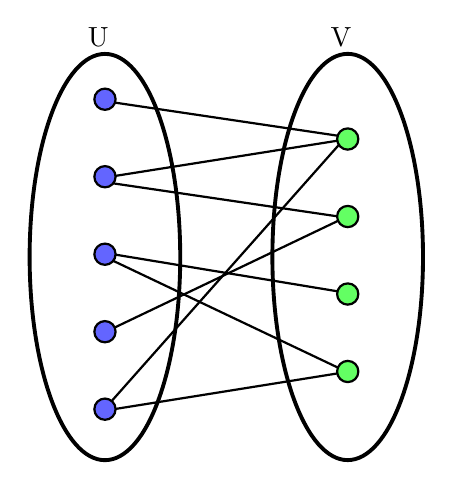
\begin{tikzpicture}[y=0.80pt, x=0.8pt,yscale=-0.5, xscale=0.5, inner sep=0pt, outer sep=0pt]
  \path[draw=black,line join=miter,line cap=butt,line width=0.800pt]
    (215.1625,381.6209) -- (421.2336,411.9255);
  \path[draw=black,line join=miter,line cap=butt,line width=0.800pt]
    (215.1625,586.4293) -- (428.3047,552.3367);
  \path[draw=black,line join=miter,line cap=butt,line width=0.800pt]
    (214.4049,445.5130) -- (428.5572,480.8684);
  \path[cm={{0.60283819,0.0,0.0,0.45550315,(91.98136,196.91071)}},draw=black,miter
    limit=4.00,line width=1.400pt] (308.5714,552.3622)arc(0.000:180.000:112.857140
    and 402.857)arc(-180.000:0.000:112.857140 and 402.857) -- cycle;
  \path[fill=black] (194.56386,258.44788) node[above right] (text3882) {U};
  \path[cm={{0.60283819,0.0,0.0,0.45550315,(311.29018,196.86231)}},draw=black,miter
    limit=4.00,line width=1.400pt] (308.5714,552.3622)arc(0.000:180.000:112.857140
    and 402.857)arc(-180.000:0.000:112.857140 and 402.857) -- cycle;
  \path[fill=black] (413.87268,258.39948) node[above right] (text3882-9) {V};
  \path[shift={(270.20979,112.61677)},draw=black,fill=c63ff63,miter
    limit=4.00,line width=0.800pt]
    (168.6955,299.2935)arc(0.000:180.000:9.596)arc(-180.000:0.000:9.596) -- cycle;
  \path[shift={(270.20979,252.61677)},draw=black,fill=c63ff63,miter
    limit=4.00,line width=0.800pt]
    (168.6955,299.2935)arc(0.000:180.000:9.596)arc(-180.000:0.000:9.596) -- cycle;
  \path[shift={(270.20979,182.61677)},draw=black,fill=c63ff63,miter
    limit=4.00,line width=0.800pt]
    (168.6955,299.2935)arc(0.000:180.000:9.596)arc(-180.000:0.000:9.596) -- cycle;
  \path[draw=black,line join=miter,line cap=butt,line width=0.800pt]
    (218.1929,308.8899) -- (422.2438,339.1945);
  \path[draw=black,line join=miter,line cap=butt,line width=0.800pt]
    (217.1828,375.5600) -- (421.2336,343.2351);
  \path[draw=black,line join=miter,line cap=butt,line width=0.800pt]
    (216.1726,451.3214) -- (420.2235,548.2961);
  \path[draw=black,line join=miter,line cap=butt,line width=0.800pt]
    (217.1828,512.9407) -- (420.2235,415.9661);
  \path[draw=black,line join=miter,line cap=butt,line width=0.800pt]
    (215.1625,579.6108) -- (421.2336,347.2757);
  \path[shift={(270.20979,42.616767)},draw=black,fill=c63ff63,miter
    limit=4.00,line width=0.800pt]
    (168.6955,299.2935)arc(0.000:180.000:9.596)arc(-180.000:0.000:9.596) -- cycle;
  \path[shift={(50.90097,6.665179)},draw=black,fill=c6365ff,miter limit=4.00,line
    width=0.800pt]
    (168.6955,299.2935)arc(0.000:180.000:9.596)arc(-180.000:0.000:9.596) -- cycle;
  \path[shift={(50.90097,76.665178)},draw=black,fill=c6365ff,miter limit=4.00,line
    width=0.800pt]
    (168.6955,299.2935)arc(0.000:180.000:9.596)arc(-180.000:0.000:9.596) -- cycle;
  \path[shift={(50.90097,146.66517)},draw=black,fill=c6365ff,miter limit=4.00,line
    width=0.800pt]
    (168.6955,299.2935)arc(0.000:180.000:9.596)arc(-180.000:0.000:9.596) -- cycle;
  \path[shift={(50.90097,216.66517)},draw=black,fill=c6365ff,miter limit=4.00,line
    width=0.800pt]
    (168.6955,299.2935)arc(0.000:180.000:9.596)arc(-180.000:0.000:9.596) -- cycle;
  \path[shift={(50.90097,286.66517)},draw=black,fill=c6365ff,miter limit=4.00,line
    width=0.800pt]
    (168.6955,299.2935)arc(0.000:180.000:9.596)arc(-180.000:0.000:9.596) -- cycle;

\end{tikzpicture}

  \caption{A sample bipartite graph}
\end{figure}

A bipartite graph is a graph in which nodes can be divided into two
node sets such that each node is only connected to nodes in the set
other than its own.

This model is able to generate realistic networks with \emph{low
  average path length}, \emph{high clustering coefficient} and
\emph{power law distribution}. The properties of the generated
networks depend solely on the distribution of edges in the bipartite
graph.

\noindent The algorithm constructs a network in three steps:
\begin{enumerate}
  \item generate a bipartite graph with two node sets, set $U$ and set
    $V$,
  \item connect all nodes in $U$ that are connected to the same node
    in $V$, and
  \item remove the nodes of set $V$ from the graph.
\end{enumerate}

\noindent In pseudocode, this looks as follows:
\begin{enumerate}
  \item Generate two node sets $U$ and $V$, with respective sizes
    $|U|$ and $|V|$:

    \begin{algorithmic}
      \REQUIRE $|U| > 0$
      \REQUIRE $|V| > 0$

      \FOR{$i=0 \to |U|$}
        \STATE add new node to $U$
      \ENDFOR

      \FOR{$i=0 \to |V|$}
        \STATE add new node to $V$
      \ENDFOR
    \end{algorithmic}

  \item For each member of $V$, calculate its scale-free degree
    distribution (see Section \ref{sec:scale-free}), and connect it to as
    many random nodes in $U$.

    \begin{algorithmic}
      \FORALL{node $v \in V$}
        \STATE $P_v \gets$ scale free distribution of $v$
        \FOR{$i=0 \to P_v$}
          \STATE $u \gets $ random node in $U$
          \STATE connect $u$ to $v$
        \ENDFOR
      \ENDFOR
    \end{algorithmic}

  \item Connect any members of $U$ which are disjoint to the network
    to a random member of $V$.

    \begin{algorithmic}
      \STATE $v \gets$ random node in $V$
      \FORALL{node $u \in U$}
        \IF{$u$ not connected to any $v \in V$}
          \STATE connect $u$ to $v$
        \ENDIF
      \ENDFOR
    \end{algorithmic}

  \item Generate sets $S_v$, which hold the edges that connect nodes
    in $U$ to the same member $v \in V$:

  \begin{algorithmic}
    \FORALL{node $v \in V$}
      \FORALL{node $u \in U$}
        \IF{$u$ is connected to $v$ by $e$}
          \STATE add $e$ to $S_v$
        \ENDIF
      \ENDFOR
    \ENDFOR
  \end{algorithmic}

  \item For all edges in sets $S_v$, connect each pair of nodes in
    $U$.

  \begin{algorithmic}
    \FORALL{node $v \in V$}
      \FORALL{edge $e_1 \in S_v$}
        \FORALL{edge $e_2 \in S_v$}
          \STATE connect nodes of $e_1$, $e_2$ not in $V$
        \ENDFOR
      \ENDFOR
    \ENDFOR
  \end{algorithmic}

  \item Remove all nodes in $V$ and all connecting edges to them.

    \begin{algorithmic}
      \FORALL{node $v \in V$}
        \FORALL{node $u \in U$}
          \IF{$u$ connected to $v$}
            \STATE disconnect $u$ from $v$
          \ENDIF
        \ENDFOR
        \STATE remove $v$ from $V$
      \ENDFOR
    \end{algorithmic}

\end{enumerate}

\subsection{Preferential attachment with clustering}

Preferential attachment and clustering are two distinct concepts used
in graph generation.

When using \emph{preferential attachment} we assign nodes a preference
depending on their degree. Nodes with more edges will have a higher
preference than nodes with fewer edges. The preference lies within the
range $[0,1]$ and, assuming that no disjoint nodes exist, is
\[ \frac{k_n}{|E|} \]
for a certain node $n$ with degree $k_n$, and $|E|$ being the total
number of edges.

\emph{Clustering} is a concept which determines how to connect a node
$n$ once a connection with at least one other node $n'$ has been
established. This procedure determines the intersection set of $n'$
with all its neighbours. Node $n$ is then connected to all members of
the intersection set.

The Barab\'{a}si-Albert model has been used frequently to model real
networks. A simple adaptation of it increases the clustering whilst
retaining the power law degree distribution of generated networks.

The bipartite nature of real networks can be interpreted as a
tendency for cliques to form in real networks. \emph{Cliques} are
fully connected subsets of vertices of a graph. Their presence
greatly increases the clustering coefficient of a network.

In the original Barab\'{a}si-Albert model, a new vertex is added to
the network by preferential attachment to a fixed number of
vertices, whereas the algorithm described in \cite{oconn11} combines
both concepts to generate networks with scale-free characteristics.

First, nodes are added to the network via the preferential attachment
method. Once attached they are connected to the rest of the
network via the clustering procedure.

\noindent So, in order to a attach a \emph{new node}, $n$,

\begin{enumerate}
  \item We will store nodes in an array alongside their
    preference. Since the preferences are stored cumulatively, a
    random number will index a particular node in the array.

  \item Generate a random percentage and find the indexed
    node\footnote{we used binary search in Visigoth, but any search
      algorithm will do}.

    \begin{algorithmic}
      \STATE $r \gets$ random percentage
      \STATE $m \gets$ node indexed by $r$
    \end{algorithmic}

  \item Attach the new node to the indexed node.

    \begin{algorithmic}
      \STATE connect $n$ to $m$
    \end{algorithmic}

   \item Use the clustering procedure to determine other edges.

    \begin{algorithmic}
      \REQUIRE Edge count with amount of edges to be added, $e$.

      \STATE $ns \gets$ neighbours($n$)

      \WHILE{$e > 0$}
        \IF{$ns$ is empty}
          \STATE \emph{break}
        \ENDIF

        \STATE $r$ $\gets$ random integer $\bmod$ size($ns$)
        \STATE node $n_r \gets ns[rand]$
        \IF{$n$ not connected to $n_r$}
          \STATE connect $n$ to $n_r$
          \STATE $e \gets e - 1$
          \STATE $ns \gets$  intersection($ns$, neighbours($n_r$))
        \ELSE
          \STATE remove $ns[$rand$]$
        \ENDIF
      \ENDWHILE
    \end{algorithmic}
\end{enumerate}

To generate a complete network of $N$ nodes, one need simply repeat
the above procedure $N$ times.


\subsection{Real small world networks}
Finally, as Visigoth is supposed to help in analysing Small World
Networks, it can also fetch real world data from the ``live'' social
networks \Twitter and \texttt{identi.ca}.



\section{Statistics}
In addition to network generation Visigoth also calculates statistics about the
generated networks in real time. The statistics which are calculated are:

\begin{itemize}
  \item Average Degree
  \item Average Path Length
  \item Clustering Average
  \item Scale Free Exponent
  \item Clustering Coefficient
\end{itemize}


\subsection{Average degree}

As explained before, in ``The maths" sections, to calculate the
average degree all degrees are summed and divided by the total number
of nodes in the network:

\begin{equation}
\ d_{avg} =\frac{\sum_{i=1}^gd(n_i)}{g}
\end{equation}
where \(g\) is the total number of nodes in the network.

Implementation is trivial.


\subsection{Average distance}
\[ \frac{\sum_{i,j}distance(n_i,n_j)}
        {\sum nodes^2 - \sum nodes}
\]

The algorithm is implemented as follows:

\begin{enumerate}

\item Calculate the sum of the distances from every node to every
node:

\begin{algorithmic}
  \FORALL{nodes $n$}
    \STATE cumulativeLength $\gets$ lengthSum(n,visited,distance)
    \STATE \dots
  \ENDFOR
\end{algorithmic}

\item Divide the calculation by $|N| \cdot (|N| - 1)$:

\begin{algorithmic}
  \RETURN $\frac{\mathrm{cumulativeLength}}{|N| \cdot (|N| - 1)}$
\end{algorithmic}

Here \code{lengthSum} is a subprocedure which traverses the network in a
breadth-first manner and calculates the distance to each node.

\item Return the sum of all distances:

\begin{algorithmic}
  \REQUIRE Starting node parent
  \REQUIRE Queue of nodes adjecent to parent
  \REQUIRE An array of visited nodes called visited
  \REQUIRE A distance array
  \WHILE{Queue is not empty}
    \STATE parent $\gets$ queue.dequeue()
    \STATE edges $\gets$ parent.edges()
    \FORALL{edge $e$}
    \STATE Node n $\gets$ e.getDifferentFromParent()
      \IF{!visited.contain(n)}
        \STATE visited.insert(n)
        \STATE distance[n] $\gets$ distance.value(parent, 0) + 1
        \STATE queue.enqueue(n)
      \ENDIF
    \ENDFOR
    \STATE retLength = retLength distance[parent]
  \ENDWHILE

  \RETURN retLength
\end{algorithmic}

\end{enumerate}

\subsection{Clustering coefficient}
As described in ``The maths" section \label{sec:clusteringcoefficient}, the
clustering coefficient $C_i$ is defined as
\[ C_i = \frac{2 \cdot |E_i|}{k_i \cdot (k_i-1)} \]

where $k_i$ is the number of neighbours of node $n_i$, $|E_i|$ is the number of edges between the neighbours of node $n_i$.

\begin{enumerate}
\item Calculate the intersection of the neighbours of the node:

We want to calculate the statistics for the node and it's neighbours:

\begin{algorithmic}
  \REQUIRE A node $n$
  \REQUIRE An edge array with edges connected to $n$
  \REQUIRE A counter called intersection
  \WHILE {!edges.empty}
    \STATE Edge $e$ $\gets$ edges.takeFirst
    \STATE Vector nNeighbours = $n$.neighbours
    \STATE Node $n_i \gets$ $e$.differentFrom($n_i$)
    \STATE Vector otherNeighbours $\gets$ $n_i$.neighbours
    \STATE intersection = intersection + intersectionCount(nNeighbours, otherNeighbours);
  \ENDWHILE
\end{algorithmic}

\item If the degree of the node is greater than 1 we return the calculation:

\begin{algorithmic}
  \REQUIRE k = n.degree
  \IF{$k > 1$}
    \RETURN $\frac{2 \cdot intersection}{k \cdot (k-1)}$
  \ELSE
    \RETURN $0$
  \ENDIF
\end{algorithmic}

\end{enumerate}

\subsection{Clustering average}

Recall from ``The maths":

\[ C_\mathrm{avg} =
   \frac{1}{\mathrm{|N|}}\sum_{i=1}^{\mathrm{|N|}} C_i
\]

\noindent where \(N\) is the total number of nodes in the graph.

This calculation is implemented as follows:

\begin{algorithmic}
  \FORALL {node $n$}
    \STATE clusterCumulative = clusterCumulative + clusteringCoeff(n)
  \ENDFOR
  \RETURN $\frac{clusterCumulative}{|N|}$
\end{algorithmic}


\subsection{Scale free exponent}
Before being able to calculate any gradient Visigoth has to probe the network
and determine the degree distribution. Since we are dealing with exponential
growth the algorithm takes the natural logarithm of both the degree and its
frequency in the network, allowing for the gradient to be calculated as a
straight line:
\[ f(x) = ax^k \equiv ln(f(x)) = kln(a) + kln(x) \equiv y = mx + b \]

The implementation we approached is:

\begin{algorithmic}
  \REQUIRE maxDegree which holds the maximum degree of the network
  \REQUIRE A vector to hold objects of type point
  \FOR { $i = 0 \to maxDegree$}
    \STATE i = i + 1
    \STATE count $\gets$ graph.nodesWithDegree(i)
    \STATE y = $\frac{count}{|N|}$
    \IF { $y \ne 0$}
      \STATE  point p($ln(i+1)$,$ln(y)$)
      \STATE plot.add(p)
    \ENDIF
  \ENDFOR
\end{algorithmic}

After recording the degree distribution the algorithm proceeds to
calculate the straight line gradient of the captured points.

\begin{algorithmic}
  \REQUIRE A vector to hold objects of type point
  \REQUIRE A counter c
  \STATE $c = 0$
  \FORALL {point $p \in$ Plot}
    \IF { $c = 0$ }
      \STATE yPrev $\gets$ p.Y
      \STATE deltaX $\gets$ p.X
    \ELSE
      \STATE deltaX = deltaX + p.Y - yPrev
      \STATE yPrev $\gets$ p.Y
      \STATE deltaX $\gets$ p.X - deltaX
    \ENDIF
      \STATE c = c + 1
  \ENDFOR
  \RETURN $- \frac{deltaY}{deltaX}$
\end{algorithmic}

The result is multiplied by -1 since the straight line
gradient is sloped downwards.




\section{Visigoth technologies}

\subsection{\Qt}

The UI toolkit, standard library replacement, and application
framework Visigoth uses is \Qt\footnote{\myhref{qt.nokia.com}}.

Visigoth relies heavily on some of \Qt's features:
\begin{description}
\item [gui] \Qt is famous for providing a cross-platform, high-level,
  UI toolkit that automatically uses the native drawing systems on
  each host platform. All of Visigoth's user visible interface was
  built using this framework. A more detailed explanation is included
  in Section \ref{gui};
\item [meta-objects] \Qt supplements the venerable \buzz{C}
  pre-processor\footnote{\myhref{gcc.gnu.org/onlinedocs/cpp}}
  with its own \buzz{meta-object
    compiler} \footnote{\myhref{developer.qt.nokia.com/doc/qt-4.8/moc.html}}.
  This preprocessor augments normal \buzz{C++} objects with modern
  features such as introspection and \code{signal}s. We use
  introspection extensively in our tests; see Section \ref{tests}. We
  use \code{signal}s to decouple objects, which leads to a cleaner
  design and has the side-effect of simplifying writing test cases
  (mock and stub objects are not necessary anymore); for details, see
  Section \ref{interaction};
\item [xml] Like most modern frameworks, \Qt provides an \buzz{XML}
  parsing
  library\footnote{\myhref{developer.qt.nokia.com/doc/qt-4.8/qtxml.html}}.
  In addition to a standard \buzz{SAX} parser, it exposes an extremely
  clean \buzz{HTML DOM}-like interface for manipulating \buzz{XML}
  documents. We use it in order to parse results from queries to
  online sources such as \Twitter and
  \href{http://identi.ca}{Identi.ca};
\item [containers] \Qt provides a fully-featured library of containers
  similar to Java
  \buzz{collections}\footnote{\myhref{docs.oracle.com/javase/1.5.0/docs/api/java/util/package-summary.html}}
  and significantly more complete than the standard or SGI
  \buzz{STL}\footnote{\myhref{www.sgi.com/tech/stl}}. The
  availability of these meant that advanced data-structures were one
  less concern to worry about during development;
\item [concurrency] \Qt also provides high-level
  threading\footnote{\myhref{developer.qt.nokia.com/doc/qt-4.8/threads.html}}
  and
  concurrency\footnote{\myhref{developer.qt.nokia.com/doc/qt-4.8/threads-qtconcurrent.html}}
  APIs. Our experiments showed that separating the CPU-intensive
  computations (e.g. generating new networks, calculating layout
  positions) onto a separate thread could speed up certain operations
  by as much as a factor of $6$. The concurrency API, which provides
  functional programming style parallelized primitives
  (e.g. \code{map}, \code{filter}) could further improve performance.
  This is an area where further work could be done in Visigoth.
\end{description}

\subsubsection{Plugins}

\Qt has a healthy plugin ecosystems, with a myriad of libraries
available to plug into the main framework. We make use of two of
these, namely
\buzz{QCA}\footnote{\myhref{delta.affinix.com/qca}} and
\buzz{QOAuth}\footnote{\href{https://github.com/ayoy/qoauth/wiki}{github.com/ayoy/qoauth/wiki}}.

\begin{description}
\item [QCA] The \buzz{Qt Cryptographic Architecture} includes many
  security providers for \Qt applications. We used the \buzz{OpenSSL}
  provider when establishing \buzz{TLS}-secured channels to the online
  sources (e.g. \Twitter);
\item [QOAuth] This library is an implementation of the \buzz{OAuth
  2.0}\footnote{\myhref{oauth.net}} secure API authorization
  standard (\buzz{OAuth} is becoming the de-facto authorization
  mechanism on the web); again, this was required in order to
  authenticate with the online sources.
\end{description}

\subsubsection{Cross-platform}

Thanks to \Qt's cross-platform nature, in general, and to
\buzz{qmake}\footnote{\myhref{developer.qt.nokia.com/doc/qt-4.8/qmake-manual.html}},
in particular, Visigoth works on Windows, OSX and Linux with a minimum
of fuss on the development side.

\begin{description}
\item [qmake] \Qt's build system, \buzz{qmake}, takes a high level
  project description and outputs platform-specific build files
  (\buzz{Makefile}s on Linux, \buzz{XCode} projects on OSX and
  \buzz{Visual Studio} projects on Windows). It also simplifies
  finding external libraries (by using its own mechanism on Linux,
  \buzz{pkg-config} on OSX, and the registry on Windows).
\end{description}

The only tweaks necessary for Visigoth to build on each of the above
platforms are a few defines to deal with the misplaced \OpenGL headers
on OSX and few conditionals in the project description to handle the
library finding on Windows.

%% FIXME: add screenshots

\subsubsection{Rapid prototyping}

One of lesser known advantages to using \Qt we discovered is rapid
prototyping. Point in case, the original prototype for Visigoth took
two days to write. It included roughly half of the customer's
\emph{must-have} features, was cross-platform and was visually
impressive.

\subsection{\OpenGL}
\label{opengl}

After being left unsatisfied with the performance achieved with a
screen renderer using \Qt graphics primitives, we looked for a
`bare-metal' graphics output solution in order to eliminate the
graphics bottleneck. Thanks to \OpenGL\footnote{\OpenGL
  documentation: https://www.opengl.org/documentation/}, we can now
draw even large graphs very quickly, no matter whether in 2D or in 3D.

\OpenGL itself is a graphics drawing interface commonly used to
leverage hardware acceleration for common operations, such as vector
transformations necessary to compute 3D graphics. Modern operating
systems use it to animate their user interfaces smoothly, and games
and professional \buzz{CAD}\footnote{Computer Assisted Design}
applications have long used it for real-time 3D graphics interaction.

Not only are we leveraging this power to speed up our graph
visualiser, but this may also allow for ports to other
platforms in the future. Thanks to the \Qt/\OpenGL base, Visigoth
could theoretically be compiled for mobile phones and slates
with minimal porting effort.

\OpenGL made several extensions possible, as outlined in the following
subsections.

\subsubsection{3D graphs and camera}
\OpenGL provides only the very fundamental drawing primitives like
lines and points --- however, it includes hardware acceleration for
vector transformations. This allows the implementation of a virtual 3D
space through which a `camera' can move. As even this is actually a
composite functionality, we wrote a helper code library
(\code{glAncillary}) to provide us with easy camera transformation
functions. They are used whenever the user decides to move around the
graph (i.e. to pan or tilt).

\subsubsection{Selection}
The \OpenGL interface also eases object selection: Since it is
responsible for the depth transformations when drawing the graphics,
it can also perform the inverse of these transformations from any
given point on the drawing surface, finding the original point in
space. In this case we check the position the mouse pointer is at and
find the object selected by the user. This is fundamental in allowing
us to move nodes around and selecting them for statistical analysis.

\subsection{\buzz{C++}}

Visigoth, ignoring the \buzz{XML} files describing the interface, is
entirely written in \buzz{C++}. Initially, while being conscious of
its disadvantages, we made this decision for one reason ---
\buzz{\Qt}. As described in the previous section, the library by Nokia
is so convenient that alone justifies the use of \buzz{C++} over
another safer language.

All in all, we think it was the right decision. The appreciation of
\buzz{C++} varies in our team, but looking back we are confident that
\buzz{C++} was one of the best choices considering the nature of the
application we have been developing.

The main advantages were:

\begin{description}

\item [Availability of tools and library] As mentioned, \Qt alone was
  a deal sealer, but the fact that we were able to access \OpenGL
  `natively' (in a \Qt widget) was also a big advantage. While
  interfaces to both libraries exist in other languages as well, we
  felt that sticking to \Qt's `native' \buzz{C++} environment would be
  the most stable solution and that the foreign language bindings
  would have degraded performance.

\item [Performance] We did not consider this factor at the beginning,
  but a few weeks into the project we started hitting various
  bottlenecks. We can only speculate about actual performance gains,
  but the fact that we were using \buzz{C++} allowed us to fine-tune
  the application (specifically on the memory management side) in a
  way that we would not be able to do with managed
  languages. Furthermore, having an optimising compiler instead of an
  interpreter or JIT (as it would have been the case using a language
  like Python or Ruby) aided performance as well.

\item [Abstraction] The previous two points (especially the second)
  are partly shared by \buzz{C++} with its predecessor,
  \buzz{C}. However, the possibility to structure our code into
  classes facilitates greatly structuring a medium sized application
  like Visigoth, especially considering that we had to coordinate five
  people working together.  For example, there is a common
  \code{Algorithm} interface which all graph generation algorithms
  have to implement. They can then be plugged into the main widget at
  will: this kind of operation would have been much more laborious and
  less type-safe in \buzz{C}.

\end{description}

However, \buzz{C++} also has its downsides:

\begin{description}

\item [Unmanaged memory] This is by far \buzz{C++}'s most
  ``dangerous'' feature (or better, lack of feature). While enabling
  greater control and thus greater performance, it requires a much
  more attentive analysis of the code. This is, in a way, a good
  thing, since it forces the programmer to reason more about what the
  code is doing; but it also paves the way to a nasty class of bugs
  and memory leaks that more than once took hours (in one case days)
  to track down. This is a somewhat controversial subject in our team
  as well as the broader programming community and our opinions differ
  on how much better a garbage collected language would have been when
  considering the loss in performance. \buzz{C++} also has the
  characteristic (required by its unmanaged nature) of allowing
  objects to be used in the heap through pointers and on the stack as
  values, which slows down compilation considerably - when changing a
  header file, all code that uses that object as a value has to be
  recompiled. Moreover, \buzz{C++} allows two kinds of references:
  immutable references and \buzz{C}-style pointers, the former with a
  rather confusing syntax - references are indistinguishable from
  values when used. All these factors generate much confusion which is
  absent in most modern O-O languages.

\item [Language bloat] \buzz{C++} is a very broad language with a
  number of esoteric language features. Notable examples are
  templates, operator overloading and ``friend'' attributes. Some of
  them are very useful and never harmful, e.g. the \code{const}
  keyword is a great mechanism to mark immutability at type
  level. However, some of them can and have been misused\footnote{For
    an hilarious example, see
    \myhref{weegen.home.xs4all.nl/eelis/analogliterals.xhtml}},
  and as a consequence,
  \begin{quote}
    ``When you're programming \buzz{C++}, no one can ever agree on
    which ten percent of the language is safe to use.'' -- Jamie
    Zawinski
  \end{quote}
  This kind of ``programming language discipline''
  is required when working on a \buzz{C++} project and we had our fair
  share of arguments on which subset of the language is safe to use;
  nevertheless we think we have managed to keep the code clean to high
  standards in the \buzz{C++} world.

\end{description}



\section{Engineering Visigoth}
%% This section corresponds to C in the requirements

We encountered a number of difficulties whilst building Visigoth,
which we overcame by dividing the application into mostly-independent
components. The following sections provide overviews and short
descriptions for each component.

\subsection{Components}
\label{components}
%% This is an overview of the classes (including a class diagram).

The \emph{[mostly]} independent components of Visigoth are:
\begin{description}
  \item [tests] The test system is heavily oriented towards
    functionality testing, checking that user actions cause the
    expected behaviour. For more details on the testing methodology,
    see Section \ref{tests};

  \item [GUI] The GUI is the only user-visible component. It was
    relies heavily on \Qt's widget library and \OpenGL. A brief
    description of the UI is provided in Section \ref{gui}, and a
    brief overview of the issues surrounding the 3D renderer can be
    found in Section \ref{opengl};

  \item [GraphScene] We took an \buzz{Model-View-Controller} approach
    in Visigoth's design. Whist the GUI system is the \buzz{view}, the
    \code{GraphScene} is the \buzz{model} and encapsulates the
    \buzz{controller}. For a brief description on how it is used, see
    Section \ref{interaction};

  \item [Algorithms] The last component of Visigoth are the algorithms. These
    were described in Section \ref{sec:algos}. All the individual algorithms
    implement the \code{Algorithm} interface, which allows them to be easily
    plugged into the \code{GraphScene}.
\end{description}

A bare-bones class diagram of the above components is include in
Figure \ref{fig:classes}. Since the internal workings of the classes
are unlikely to be of interest to the reader and to highlight the
relationships between components, we only include inheritance and
usages.

\begin{figure}[ht!]
  \centering
  
\definecolor{c2b1100}{RGB}{43,17,0}

\begin{tikzpicture}[y=0.80pt, x=0.8pt,yscale=-1, inner sep=0pt, outer sep=0pt]
\begin{scope}[shift={(-174.90031,-221.35276)}]
    \path[cm={{1.0,0.0,-0.25881906,0.96592582,(0.0,0.0)}},draw=c2b1100,line
      join=miter,line cap=butt,miter limit=4.00,line width=0.814pt,rounded
      corners=0.0000cm] (519.1957,689.8035) rectangle (588.3925,706.1153);
    \path[cm={{1.0,0.0,-0.26794921,1.0,(0.0,0.0)}},fill=black] (527.67328,682.25549)
      node[above right] (text2987) {Algorithm     };
    \path[fill=black] (496.41861,726.57574) node[above right] (text3043) {Twitter
      };
    \path[draw=c2b1100,line join=miter,line cap=butt,miter limit=4.00,line
      width=0.800pt,rounded corners=0.0000cm] (492.9985,713.3670) rectangle
      (540.3671,729.1670);
    \path[fill=black] (211.3568,728.34882) node[above right] (text3007) {ErdosRenyi
      };
    \path[draw=c2b1100,line join=miter,line cap=butt,miter limit=4.00,line
      width=0.800pt,rounded corners=0.0000cm] (205.9307,713.3976) rectangle
      (280.2136,729.1363);
    \path[fill=black] (233.92371,751.40686) node[above right] (text2991)
      {BarabasiAlbert       };
    \path[draw=c2b1100,line join=miter,line cap=butt,miter limit=4.00,line
      width=0.800pt,rounded corners=0.0000cm] (227.7710,738.1706) rectangle
      (321.1261,754.0257);
    \path[fill=black] (434.84686,752.258) node[above right] (text3055)
      {WattsStrogatz       };
    \path[draw=c2b1100,line join=miter,line cap=butt,miter limit=4.00,line
      width=0.800pt,rounded corners=0.0000cm] (427.4141,738.1981) rectangle
      (518.5268,753.9981);
    \path[fill=black] (304.90619,774.91241) node[above right] (text2999) {Bipartite
      };
    \path[draw=c2b1100,line join=miter,line cap=butt,miter limit=4.00,line
      width=0.800pt,rounded corners=0.0000cm] (298.3260,760.8566) rectangle
      (356.7958,776.6545);
    \path[fill=black] (380.16458,774.13904) node[above right] (text3027)
      {Preferential       };
    \path[draw=c2b1100,line join=miter,line cap=butt,miter limit=4.00,line
      width=0.800pt,rounded corners=0.0000cm] (375.0404,760.8328) rectangle
      (447.9719,776.6782);
  \path[draw=c2b1100,line join=miter,line cap=butt,miter limit=4.00,line
    width=0.800pt,rounded corners=0.0000cm] (185.4003,637.4907) rectangle
    (560.8975,787.1140);
  \path[fill=black] (344.63321,651.64423) node[above right] (text8048) {Algorithm
    };
    \path[fill=black] (338.94666,553.91602) node[above right] (text3015) {GraphScene
      };
    \path[draw=c2b1100,line join=miter,line cap=butt,miter limit=4.00,line
      width=0.800pt,rounded corners=0.0000cm] (334.7563,539.7668) rectangle
      (412.0519,555.6020);
    \path[fill=black] (445.23074,604.19696) node[above right] (text3003) {Edge
      };
    \path[draw=c2b1100,line join=miter,line cap=butt,miter limit=4.00,line
      width=0.800pt,rounded corners=0.0000cm] (434.5910,589.2089) rectangle
      (484.8885,605.0215);
    \path[fill=black] (370.77048,602.49573) node[above right] (text3035) {Statistics
      };
    \path[draw=c2b1100,line join=miter,line cap=butt,miter limit=4.00,line
      width=0.800pt,rounded corners=0.0000cm] (367.9417,589.1925) rectangle
      (422.6464,605.0379);
    \path[fill=black] (500.56403,602.42395) node[above right] (text3023) {Node
      };
    \path[draw=c2b1100,line join=miter,line cap=butt,miter limit=4.00,line
      width=0.800pt,rounded corners=0.0000cm] (496.8331,589.2151) rectangle
      (533.9948,605.0152);
    \path[fill=black] (295.83789,604.22595) node[above right] (text3031) {QuadTree
      };
    \path[draw=c2b1100,line join=miter,line cap=butt,miter limit=4.00,line
      width=0.800pt,rounded corners=0.0000cm] (290.3776,589.2031) rectangle
      (355.9972,605.0273);
  \path[fill=black] (337.25412,525.9975) node[above right] (text8260) {GraphScene
    };
  \path[draw=c2b1100,line join=miter,line cap=butt,miter limit=4.00,line
    width=0.800pt,rounded corners=0.0000cm] (185.4003,512.3205) rectangle
    (561.4079,617.3446);
    \path[fill=black] (217.17059,603.20026) node[above right] (text8178) {Algorithm
      };
    \path[draw=c2b1100,line join=miter,line cap=butt,miter limit=4.00,line
      width=0.800pt,rounded corners=0.0000cm] (212.8134,589.2031) rectangle
      (278.4330,605.0273);
    \path[draw=c2b1100,line join=miter,line cap=butt,miter limit=4.00,line
      width=0.725pt] (209.3740,589.9500) .. controls (209.3740,596.9025) and
      (209.3740,603.8551) .. (209.3740,610.8077) .. controls (233.5418,610.8077) and
      (257.7095,610.8077) .. (281.8773,610.8077) .. controls (281.8773,601.6821) and
      (281.8773,592.5566) .. (281.8773,583.4310) .. controls (257.7096,583.4310) and
      (233.5418,583.4310) .. (209.3740,583.4310) .. controls (209.3740,585.6040) and
      (209.3740,587.7770) .. (209.3740,589.9500) -- cycle;
    \path[fill=black] (349.01846,364.20969) node[above right] (text3019) {MainWindow
      };
    \path[draw=c2b1100,line join=miter,line cap=butt,miter limit=4.00,line
      width=0.800pt,rounded corners=0.0000cm] (341.0906,350.1661) rectangle
      (427.8468,367.6358);
    \path[fill=black] (344.43729,334.3941) node[above right] (text3993) {QMainWindow
      };
    \path[draw=c2b1100,line join=miter,line cap=butt,miter limit=4.00,line
      width=0.800pt,rounded corners=0.0000cm] (334.8936,319.6544) rectangle
      (434.0439,336.9058);
    \path[fill=black] (282.29581,441.0975) node[above right] (text3011)
      {GLGraphWidget       };
    \path[draw=c2b1100,line join=miter,line cap=butt,miter limit=4.00,line
      width=0.800pt,rounded corners=0.0000cm] (272.9869,426.2390) rectangle
      (380.6145,443.6365);
    \path[fill=black] (266.82867,478.84314) node[above right] (text3047) {VCubeF
      };
    \path[draw=c2b1100,line join=miter,line cap=butt,miter limit=4.00,line
      width=0.800pt,rounded corners=0.0000cm] (258.3968,465.5352) rectangle
      (319.6728,481.3902);
    \path[fill=black] (343.45309,478.77136) node[above right] (text3051) {VPointF
      };
  \path[draw=c2b1100,line join=miter,line cap=butt,miter limit=4.00,line
    width=0.800pt,rounded corners=0.0000cm] (334.7740,465.5933) rectangle
    (395.2047,481.3320);
    \path[fill=black] (244.02667,396.08804) node[above right] (text4009) {QGLWidget
      };
    \path[draw=c2b1100,line join=miter,line cap=butt,miter limit=4.00,line
      width=0.800pt,rounded corners=0.0000cm] (236.7780,381.0354) rectangle
      (314.7539,396.8218);
    \path[fill=black] (431.61746,441.0975) node[above right] (text8334) {GraphScene
      };
    \path[draw=c2b1100,line join=miter,line cap=butt,miter limit=4.00,line
      width=0.800pt,rounded corners=0.0000cm] (426.5960,426.9728) rectangle
      (505.5539,442.7592);
    \path[draw=c2b1100,line join=miter,line cap=butt,miter limit=4.00,line
      width=0.762pt] (421.5986,427.3390) .. controls (421.5986,434.6404) and
      (421.5986,441.9417) .. (421.5986,449.2431) .. controls (451.2499,449.2431) and
      (480.9013,449.2431) .. (510.5526,449.2431) .. controls (510.5526,439.6566) and
      (510.5526,430.0700) .. (510.5526,420.4835) .. controls (480.9013,420.4835) and
      (451.2499,420.4835) .. (421.5986,420.4835) .. controls (421.5986,422.7687) and
      (421.5986,425.0538) .. (421.5986,427.3390) -- cycle;
  \path[draw=c2b1100,line join=miter,line cap=butt,miter limit=4.00,line
    width=0.800pt,rounded corners=0.0000cm] (185.4003,293.6357) rectangle
    (561.9182,492.1744);
  \path[fill=black] (362.87619,305.86453) node[above right] (text9031) {GUI     };
  \path[draw=c2b1100,dash pattern=on 2.40pt off 0.80pt,line join=miter,line
    cap=butt,miter limit=4.00,line width=0.800pt,rounded corners=0.0000cm]
    (211.7161,373.8237) rectangle (402.9694,487.7619);
  \begin{scope}[cm={{0.0,-1.0,1.0,0.0,(0.0,0.0)}},fill=black]
    \path[fill] (-461.3479,205.3749) -- (-460.2714,205.2313) .. controls
      (-460.1478,205.8414) and (-459.9385,206.2819) .. (-459.6434,206.5531) ..
      controls (-459.3444,206.8202) and (-458.9816,206.9538) .. (-458.5550,206.9538)
      .. controls (-458.0486,206.9538) and (-457.6220,206.7783) ..
      (-457.2751,206.4275) .. controls (-456.9242,206.0766) and (-456.7488,205.6420)
      .. (-456.7488,205.1237) .. controls (-456.7488,204.6293) and
      (-456.9103,204.2226) .. (-457.2332,203.9037) .. controls (-457.5562,203.5807)
      and (-457.9669,203.4192) .. (-458.4652,203.4192) .. controls
      (-458.6686,203.4192) and (-458.9218,203.4591) .. (-459.2248,203.5388) --
      (-459.1052,202.5939) .. controls (-459.0334,202.6019) and (-458.9756,202.6059)
      .. (-458.9317,202.6059) .. controls (-458.4732,202.6059) and
      (-458.0605,202.4863) .. (-457.6937,202.2471) .. controls (-457.3269,202.0078)
      and (-457.1435,201.6390) .. (-457.1435,201.1406) .. controls
      (-457.1435,200.7459) and (-457.2771,200.4190) .. (-457.5442,200.1598) ..
      controls (-457.8114,199.9007) and (-458.1562,199.7711) .. (-458.5789,199.7711)
      .. controls (-458.9975,199.7711) and (-459.3464,199.9027) ..
      (-459.6255,200.1658) .. controls (-459.9046,200.4289) and (-460.0840,200.8237)
      .. (-460.1637,201.3500) -- (-461.2403,201.1586) .. controls
      (-461.1087,200.4369) and (-460.8096,199.8787) .. (-460.3432,199.4840) ..
      controls (-459.8767,199.0853) and (-459.2965,198.8859) .. (-458.6028,198.8859)
      .. controls (-458.1243,198.8859) and (-457.6838,198.9896) ..
      (-457.2811,199.1969) .. controls (-456.8784,199.4003) and (-456.5714,199.6794)
      .. (-456.3600,200.0342) .. controls (-456.1448,200.3891) and
      (-456.0371,200.7659) .. (-456.0371,201.1646) .. controls (-456.0371,201.5433)
      and (-456.1388,201.8882) .. (-456.3421,202.1992) .. controls
      (-456.5455,202.5102) and (-456.8465,202.7574) .. (-457.2452,202.9408) ..
      controls (-456.7269,203.0604) and (-456.3242,203.3096) .. (-456.0371,203.6884)
      .. controls (-455.7500,204.0632) and (-455.6065,204.5337) ..
      (-455.6065,205.0998) .. controls (-455.6065,205.8653) and (-455.8856,206.5152)
      .. (-456.4438,207.0495) .. controls (-457.0020,207.5798) and
      (-457.7077,207.8449) .. (-458.5609,207.8449) .. controls (-459.3304,207.8449)
      and (-459.9704,207.6157) .. (-460.4807,207.1572) .. controls
      (-460.9871,206.6986) and (-461.2761,206.1046) .. (-461.3479,205.3749);
    \path[fill] (-454.0994,207.6894) -- (-454.0994,198.9218) -- (-451.0792,198.9218)
      .. controls (-450.3974,198.9218) and (-449.8770,198.9637) ..
      (-449.5182,199.0474) .. controls (-449.0158,199.1630) and (-448.5872,199.3723)
      .. (-448.2324,199.6753) .. controls (-447.7699,200.0661) and
      (-447.4250,200.5665) .. (-447.1977,201.1765) .. controls (-446.9665,201.7825)
      and (-446.8508,202.4763) .. (-446.8508,203.2577) .. controls
      (-446.8508,203.9236) and (-446.9286,204.5137) .. (-447.0841,205.0280) ..
      controls (-447.2396,205.5423) and (-447.4389,205.9690) .. (-447.6821,206.3079)
      .. controls (-447.9254,206.6428) and (-448.1925,206.9079) ..
      (-448.4835,207.1033) .. controls (-448.7706,207.2947) and (-449.1195,207.4402)
      .. (-449.5302,207.5399) .. controls (-449.9368,207.6396) and
      (-450.4053,207.6894) .. (-450.9356,207.6894) --
      (-454.0994,207.6894)(-452.9391,206.6547) -- (-451.0672,206.6547) .. controls
      (-450.4891,206.6547) and (-450.0365,206.6009) .. (-449.7096,206.4933) ..
      controls (-449.3787,206.3856) and (-449.1155,206.2341) .. (-448.9201,206.0387)
      .. controls (-448.6450,205.7636) and (-448.4317,205.3948) ..
      (-448.2802,204.9323) .. controls (-448.1247,204.4658) and (-448.0470,203.9017)
      .. (-448.0470,203.2398) .. controls (-448.0470,202.3228) and
      (-448.1985,201.6191) .. (-448.5015,201.1286) .. controls (-448.8005,200.6342)
      and (-449.1653,200.3033) .. (-449.5959,200.1358) .. controls
      (-449.9069,200.0162) and (-450.4073,199.9564) .. (-451.0971,199.9564) --
      (-452.9391,199.9564) -- (-452.9391,206.6547);
    \path[fill] (-441.8570,207.6894) -- (-441.8570,198.9218) -- (-437.9696,198.9218)
      .. controls (-437.1881,198.9218) and (-436.5940,199.0015) ..
      (-436.1873,199.1610) .. controls (-435.7807,199.3165) and (-435.4557,199.5936)
      .. (-435.2125,199.9923) .. controls (-434.9693,200.3910) and
      (-434.8477,200.8316) .. (-434.8477,201.3140) .. controls (-434.8477,201.9360)
      and (-435.0490,202.4603) .. (-435.4517,202.8869) .. controls
      (-435.8544,203.3136) and (-436.4764,203.5847) .. (-437.3177,203.7003) ..
      controls (-437.0107,203.8478) and (-436.7774,203.9934) .. (-436.6180,204.1369)
      .. controls (-436.2791,204.4479) and (-435.9581,204.8366) ..
      (-435.6551,205.3031) -- (-434.1300,207.6894) -- (-435.5893,207.6894) --
      (-436.7495,205.8653) .. controls (-437.0884,205.3390) and (-437.3675,204.9363)
      .. (-437.5868,204.6572) .. controls (-437.8061,204.3781) and
      (-438.0035,204.1827) .. (-438.1789,204.0711) .. controls (-438.3504,203.9595)
      and (-438.5258,203.8817) .. (-438.7052,203.8379) .. controls
      (-438.8368,203.8100) and (-439.0521,203.7960) .. (-439.3511,203.7960) --
      (-440.6968,203.7960) -- (-440.6968,207.6894) --
      (-441.8570,207.6894)(-440.6968,202.7912) -- (-438.2028,202.7912) .. controls
      (-437.6725,202.7912) and (-437.2579,202.7374) .. (-436.9589,202.6297) ..
      controls (-436.6598,202.5181) and (-436.4326,202.3427) .. (-436.2771,202.1034)
      .. controls (-436.1216,201.8602) and (-436.0438,201.5971) ..
      (-436.0438,201.3140) .. controls (-436.0438,200.8993) and (-436.1953,200.5584)
      .. (-436.4983,200.2913) .. controls (-436.7974,200.0242) and
      (-437.2718,199.8906) .. (-437.9217,199.8906) -- (-440.6968,199.8906) --
      (-440.6968,202.7912);
    \path[fill] (-428.8132,205.6440) -- (-427.7008,205.7816) .. controls
      (-427.8763,206.4315) and (-428.2012,206.9358) .. (-428.6757,207.2947) ..
      controls (-429.1501,207.6535) and (-429.7562,207.8329) .. (-430.4938,207.8329)
      .. controls (-431.4228,207.8329) and (-432.1604,207.5479) ..
      (-432.7066,206.9777) .. controls (-433.2489,206.4036) and (-433.5200,205.6002)
      .. (-433.5200,204.5675) .. controls (-433.5200,203.4990) and
      (-433.2449,202.6697) .. (-432.6947,202.0796) .. controls (-432.1444,201.4895)
      and (-431.4308,201.1944) .. (-430.5536,201.1944) .. controls
      (-429.7043,201.1944) and (-429.0106,201.4835) .. (-428.4723,202.0616) ..
      controls (-427.9341,202.6397) and (-427.6650,203.4531) .. (-427.6649,204.5017)
      .. controls (-427.6650,204.5655) and (-427.6669,204.6612) ..
      (-427.6709,204.7888) -- (-432.4076,204.7888) .. controls (-432.3677,205.4865)
      and (-432.1704,206.0208) .. (-431.8155,206.3916) .. controls
      (-431.4607,206.7624) and (-431.0181,206.9478) .. (-430.4878,206.9478) ..
      controls (-430.0931,206.9478) and (-429.7562,206.8441) .. (-429.4771,206.6368)
      .. controls (-429.1980,206.4295) and (-428.9767,206.0985) ..
      (-428.8132,205.6440)(-432.3478,203.9036) -- (-428.8013,203.9036) .. controls
      (-428.8491,203.3694) and (-428.9847,202.9687) .. (-429.2080,202.7015) ..
      controls (-429.5509,202.2869) and (-429.9954,202.0796) .. (-430.5417,202.0795)
      .. controls (-431.0360,202.0796) and (-431.4527,202.2450) ..
      (-431.7916,202.5759) .. controls (-432.1265,202.9069) and (-432.3119,203.3494)
      .. (-432.3478,203.9036);
    \path[fill] (-426.3432,207.6894) -- (-426.3432,201.3380) -- (-425.3743,201.3380)
      -- (-425.3743,202.2410) .. controls (-424.9079,201.5433) and
      (-424.2340,201.1944) .. (-423.3529,201.1944) .. controls (-422.9701,201.1944)
      and (-422.6193,201.2642) .. (-422.3003,201.4037) .. controls
      (-421.9774,201.5393) and (-421.7361,201.7187) .. (-421.5766,201.9420) ..
      controls (-421.4172,202.1653) and (-421.3055,202.4304) .. (-421.2417,202.7374)
      .. controls (-421.2018,202.9368) and (-421.1819,203.2857) ..
      (-421.1819,203.7840) -- (-421.1819,207.6894) -- (-422.2584,207.6894) --
      (-422.2584,203.8259) .. controls (-422.2584,203.3873) and (-422.3003,203.0604)
      .. (-422.3840,202.8451) .. controls (-422.4677,202.6258) and
      (-422.6173,202.4523) .. (-422.8326,202.3248) .. controls (-423.0439,202.1932)
      and (-423.2931,202.1274) .. (-423.5802,202.1274) .. controls
      (-424.0387,202.1274) and (-424.4354,202.2729) .. (-424.7703,202.5640) ..
      controls (-425.1013,202.8550) and (-425.2667,203.4073) .. (-425.2667,204.2206)
      -- (-425.2667,207.6894) -- (-426.3432,207.6894);
    \path[fill] (-415.4046,207.6894) -- (-415.4046,206.8880) .. controls
      (-415.8073,207.5180) and (-416.3994,207.8329) .. (-417.1809,207.8329) ..
      controls (-417.6872,207.8329) and (-418.1537,207.6934) .. (-418.5803,207.4143)
      .. controls (-419.0030,207.1352) and (-419.3319,206.7464) ..
      (-419.5672,206.2481) .. controls (-419.7984,205.7457) and (-419.9140,205.1695)
      .. (-419.9140,204.5196) .. controls (-419.9140,203.8857) and
      (-419.8084,203.3116) .. (-419.5971,202.7972) .. controls (-419.3857,202.2789)
      and (-419.0688,201.8822) .. (-418.6461,201.6071) .. controls
      (-418.2235,201.3320) and (-417.7510,201.1944) .. (-417.2287,201.1944) ..
      controls (-416.8460,201.1944) and (-416.5051,201.2761) .. (-416.2060,201.4396)
      .. controls (-415.9070,201.5991) and (-415.6638,201.8084) ..
      (-415.4764,202.0676) -- (-415.4764,198.9218) -- (-414.4059,198.9218) --
      (-414.4059,207.6894) -- (-415.4046,207.6894)(-418.8076,204.5197) .. controls
      (-418.8076,205.3330) and (-418.6362,205.9411) .. (-418.2933,206.3438) ..
      controls (-417.9504,206.7465) and (-417.5457,206.9478) .. (-417.0792,206.9478)
      .. controls (-416.6087,206.9478) and (-416.2100,206.7564) ..
      (-415.8831,206.3737) .. controls (-415.5521,205.9869) and (-415.3867,205.3988)
      .. (-415.3867,204.6094) .. controls (-415.3867,203.7402) and
      (-415.5541,203.1022) .. (-415.8891,202.6956) .. controls (-416.2240,202.2889)
      and (-416.6366,202.0855) .. (-417.1270,202.0855) .. controls
      (-417.6055,202.0855) and (-418.0062,202.2809) .. (-418.3292,202.6716) ..
      controls (-418.6481,203.0624) and (-418.8076,203.6784) ..
      (-418.8076,204.5197);
    \path[fill] (-408.3834,205.6440) -- (-407.2710,205.7816) .. controls
      (-407.4464,206.4315) and (-407.7713,206.9358) .. (-408.2458,207.2947) ..
      controls (-408.7203,207.6535) and (-409.3263,207.8329) .. (-410.0639,207.8329)
      .. controls (-410.9929,207.8329) and (-411.7305,207.5479) ..
      (-412.2767,206.9777) .. controls (-412.8190,206.4036) and (-413.0901,205.6002)
      .. (-413.0901,204.5675) .. controls (-413.0901,203.4990) and
      (-412.8150,202.6697) .. (-412.2648,202.0796) .. controls (-411.7146,201.4895)
      and (-411.0009,201.1944) .. (-410.1237,201.1944) .. controls
      (-409.2745,201.1944) and (-408.5807,201.4835) .. (-408.0425,202.0616) ..
      controls (-407.5042,202.6397) and (-407.2351,203.4531) .. (-407.2351,204.5017)
      .. controls (-407.2351,204.5655) and (-407.2371,204.6612) ..
      (-407.2411,204.7888) -- (-411.9777,204.7888) .. controls (-411.9378,205.4865)
      and (-411.7405,206.0208) .. (-411.3856,206.3916) .. controls
      (-411.0308,206.7624) and (-410.5882,206.9478) .. (-410.0580,206.9478) ..
      controls (-409.6632,206.9478) and (-409.3263,206.8441) .. (-409.0472,206.6368)
      .. controls (-408.7681,206.4295) and (-408.5469,206.0985) ..
      (-408.3834,205.6440)(-411.9179,203.9036) -- (-408.3714,203.9036) .. controls
      (-408.4192,203.3694) and (-408.5548,202.9687) .. (-408.7781,202.7015) ..
      controls (-409.1210,202.2869) and (-409.5655,202.0796) .. (-410.1118,202.0795)
      .. controls (-410.6062,202.0796) and (-411.0228,202.2450) ..
      (-411.3617,202.5759) .. controls (-411.6967,202.9069) and (-411.8821,203.3494)
      .. (-411.9179,203.9036);
    \path[fill] (-405.9253,207.6894) -- (-405.9253,201.3380) -- (-404.9564,201.3380)
      -- (-404.9564,202.3008) .. controls (-404.7093,201.8503) and
      (-404.4820,201.5533) .. (-404.2747,201.4097) .. controls (-404.0633,201.2662)
      and (-403.8321,201.1944) .. (-403.5809,201.1944) .. controls
      (-403.2181,201.1944) and (-402.8493,201.3101) .. (-402.4745,201.5413) --
      (-402.8453,202.5401) .. controls (-403.1084,202.3846) and (-403.3716,202.3068)
      .. (-403.6347,202.3068) .. controls (-403.8700,202.3068) and
      (-404.0813,202.3786) .. (-404.2687,202.5221) .. controls (-404.4561,202.6617)
      and (-404.5896,202.8570) .. (-404.6694,203.1082) .. controls
      (-404.7890,203.4910) and (-404.8488,203.9096) .. (-404.8488,204.3642) --
      (-404.8488,207.6894) -- (-405.9253,207.6894);
    \path[fill] (-397.4986,205.6440) -- (-396.3862,205.7816) .. controls
      (-396.5616,206.4315) and (-396.8866,206.9358) .. (-397.3610,207.2947) ..
      controls (-397.8355,207.6535) and (-398.4415,207.8329) .. (-399.1791,207.8329)
      .. controls (-400.1081,207.8329) and (-400.8458,207.5479) ..
      (-401.3920,206.9777) .. controls (-401.9342,206.4036) and (-402.2054,205.6002)
      .. (-402.2054,204.5675) .. controls (-402.2054,203.4990) and
      (-401.9302,202.6697) .. (-401.3800,202.0796) .. controls (-400.8298,201.4895)
      and (-400.1161,201.1944) .. (-399.2389,201.1944) .. controls
      (-398.3897,201.1944) and (-397.6959,201.4835) .. (-397.1577,202.0616) ..
      controls (-396.6194,202.6397) and (-396.3503,203.4531) .. (-396.3503,204.5017)
      .. controls (-396.3503,204.5655) and (-396.3523,204.6612) ..
      (-396.3563,204.7888) -- (-401.0930,204.7888) .. controls (-401.0531,205.4865)
      and (-400.8557,206.0208) .. (-400.5009,206.3916) .. controls
      (-400.1460,206.7624) and (-399.7035,206.9478) .. (-399.1732,206.9478) ..
      controls (-398.7785,206.9478) and (-398.4416,206.8441) .. (-398.1624,206.6368)
      .. controls (-397.8834,206.4295) and (-397.6621,206.0985) ..
      (-397.4986,205.6440)(-401.0332,203.9036) -- (-397.4866,203.9036) .. controls
      (-397.5344,203.3694) and (-397.6700,202.9687) .. (-397.8933,202.7015) ..
      controls (-398.2362,202.2869) and (-398.6808,202.0796) .. (-399.2270,202.0795)
      .. controls (-399.7214,202.0796) and (-400.1381,202.2450) ..
      (-400.4770,202.5759) .. controls (-400.8119,202.9069) and (-400.9973,203.3494)
      .. (-401.0332,203.9036);
    \path[fill] (-395.0405,207.6894) -- (-395.0405,201.3380) -- (-394.0717,201.3380)
      -- (-394.0717,202.3008) .. controls (-393.8245,201.8503) and
      (-393.5972,201.5533) .. (-393.3899,201.4097) .. controls (-393.1786,201.2662)
      and (-392.9473,201.1944) .. (-392.6961,201.1944) .. controls
      (-392.3333,201.1944) and (-391.9645,201.3101) .. (-391.5897,201.5413) --
      (-391.9605,202.5401) .. controls (-392.2237,202.3846) and (-392.4868,202.3068)
      .. (-392.7500,202.3068) .. controls (-392.9852,202.3068) and
      (-393.1965,202.3786) .. (-393.3839,202.5221) .. controls (-393.5713,202.6617)
      and (-393.7049,202.8570) .. (-393.7846,203.1082) .. controls
      (-393.9042,203.4910) and (-393.9640,203.9096) .. (-393.9640,204.3642) --
      (-393.9640,207.6894) -- (-395.0405,207.6894);
  \end{scope}
  \begin{scope}[cm={{0.86518633,0.0,0.0,0.86518633,(75.812581,106.17205)}}]
    \begin{scope}[cm={{0.58987066,0.0,0.0,0.58987066,(243.55794,-118.25366)}}]
      \path[fill=black] (112.20258,519.59692) node[above right] (text3039) {TestSimple
        };
      \path[draw=c2b1100,line join=miter,line cap=butt,miter limit=4.00,line
        width=1.568pt,rounded corners=0.0000cm] (105.7002,489.9196) rectangle
        (235.7284,520.9477);
    \end{scope}
    \path[draw=c2b1100,line join=miter,line cap=butt,miter limit=4.00,line
      width=0.925pt,rounded corners=0.0000cm] (126.7476,145.2643) rectangle
      (561.7670,193.3053);
    \path[fill=black] (326.46439,160.47791) node[above right] (text9388) {Tests
      };
  \end{scope}
  \path[shift={(174.90031,221.35276)},draw=black,line join=miter,line
    cap=butt,line width=0.800pt] (106.1957,362.0783) -- (178.3086,334.2492);
  \path[shift={(174.90031,221.35276)},draw=black,line join=miter,line
    cap=butt,line width=0.800pt] (156.3452,367.8503) -- (190.5664,334.2492);
  \path[shift={(174.90031,221.35276)},draw=black,line join=miter,line
    cap=butt,line width=0.800pt] (216.8765,367.8397) -- (201.9638,334.2492);
  \path[shift={(174.90031,221.35276)},draw=black,line join=miter,line
    cap=butt,line width=0.800pt] (270.0860,367.8562) -- (211.9789,334.2492);
  \path[shift={(174.90031,221.35276)},draw=black,line join=miter,line
    cap=butt,line width=0.800pt] (321.9328,369.3110) -- (220.9501,334.2492);
  \path[shift={(174.90031,221.35276)},draw=black,line join=miter,line
    cap=butt,line width=0.800pt] (121.9058,244.1824) -- (143.3731,222.2837);
  \path[shift={(174.90031,221.35276)},draw=black,line join=miter,line
    cap=butt,line width=0.800pt] (182.2884,244.2405) -- (160.5232,222.2837);
  \path[shift={(174.90031,221.35276)},draw=black,line join=miter,line
    cap=butt,line width=0.800pt] (142.1085,204.8862) -- (108.9944,175.4690);
  \path[shift={(174.90031,221.35276)},draw=black,line join=miter,line
    cap=butt,line width=0.800pt] (158.4977,204.8862) -- (202.9437,146.2831);
  \path[shift={(174.90031,221.35276)},draw=black,line join=miter,line
    cap=butt,line width=0.800pt] (275.7270,199.1308) -- (218.9523,146.2831);
  \path[shift={(174.90031,221.35276)},draw=black,line join=miter,line
    cap=butt,line width=0.800pt] (209.5684,128.8134) -- (209.5684,115.5531);
  \path[shift={(174.90031,221.35276)},draw=black,line join=miter,line
    cap=butt,line width=0.800pt] (91.9405,492.0449) -- (179.4364,460.7022);
  \path[shift={(174.90031,221.35276)},draw=black,line join=miter,line
    cap=butt,line width=0.800pt] (110.6026,516.8178) -- (188.8517,460.7022);
  \path[shift={(174.90031,221.35276)},draw=black,line join=miter,line
    cap=butt,line width=0.800pt] (156.5572,539.5038) -- (194.9641,460.7022);
  \path[shift={(174.90031,221.35276)},draw=black,line join=miter,line
    cap=butt,line width=0.800pt] (233.3535,539.4801) -- (201.0149,460.7022);
  \path[shift={(174.90031,221.35276)},draw=black,line join=miter,line
    cap=butt,line width=0.800pt] (286.7181,516.8454) -- (207.7296,460.7022);
  \path[shift={(174.90031,221.35276)},draw=black,line join=miter,line
    cap=butt,line width=0.800pt] (318.0982,492.3319) -- (219.2985,460.7022);
\end{scope}

\end{tikzpicture}

  \caption{Class diagram for each of Visigoth's components}
  \label{fig:classes}
\end{figure}

\subsection{GUI}
\label{gui}

Since Visigoth is an end-user-oriented application, the GUI is, by
far, the most important component. Luckily, the user work-flows we
considered contain very few steps (hence, there is little need for
``Wizards'' or nested-design).

As shown in Figure \ref{fig:gui-sketch}, the Visigoth UI is
\emph{flat}. All relevant options and displays are presented to the
user in a single encompassing interface. Relevancy is determined by
context; for instance, the generation parameters shown (Figure
\ref{fig:gui-sketch}.3) vary depending on the algorithm selected (in
Figure \ref{fig:gui-sketch}.1).

\begin{figure}[ht!]
  \centering
  
\definecolor{c2b1100}{RGB}{43,17,0}

\begin{tikzpicture}[y=0.80pt, x=0.8pt,yscale=-1, inner sep=0pt, outer sep=0pt]
\begin{scope}[shift={(-235.60247,-129.32997)}]
    \path[draw=c2b1100,line join=miter,line cap=butt,miter limit=4.00,line
      width=0.800pt,rounded corners=0.0000cm] (246.1028,139.8300) rectangle
      (545.7283,376.0971);
    \path[draw=c2b1100,line join=miter,line cap=butt,miter limit=4.00,line
      width=0.800pt,rounded corners=0.0000cm] (455.1049,187.9840) rectangle
      (540.7122,212.7299);
    \path[fill=black] (495.20386,204.3949) node[above right] (text2995) {1       };
    \path[cm={{0.46816479,0.0,0.0,0.46816479,(423.67103,-163.24222)}},draw=c2b1100,line
      join=miter,line cap=butt,miter limit=4.00,line width=1.709pt]
      (174.2857,776.6479) .. controls (174.2857,785.3266) and (167.2502,792.3622) ..
      (158.5714,792.3622) .. controls (149.8927,792.3622) and (142.8571,785.3266) ..
      (142.8571,776.6479) .. controls (142.8571,767.9691) and (149.8927,760.9336) ..
      (158.5714,760.9336) .. controls (167.2502,760.9336) and (174.2857,767.9691) ..
      (174.2857,776.6479) -- cycle;
    \path[draw=c2b1100,line join=miter,line cap=butt,miter limit=4.00,line
      width=0.800pt,rounded corners=0.0000cm] (455.1021,220.4184) rectangle
      (540.7150,278.6103);
    \path[fill=black] (494.91574,253.55225) node[above right] (text3772) {2       };
    \path[cm={{0.46816479,0.0,0.0,0.46816479,(423.67096,-114.08487)}},draw=c2b1100,line
      join=miter,line cap=butt,miter limit=4.00,line width=1.709pt]
      (174.2857,776.6479) .. controls (174.2857,785.3266) and (167.2502,792.3622) ..
      (158.5714,792.3622) .. controls (149.8927,792.3622) and (142.8571,785.3266) ..
      (142.8571,776.6479) .. controls (142.8571,767.9691) and (149.8927,760.9336) ..
      (158.5714,760.9336) .. controls (167.2502,760.9336) and (174.2857,767.9691) ..
      (174.2857,776.6479) -- cycle;
    \path[draw=c2b1100,line join=miter,line cap=butt,miter limit=4.00,line
      width=0.800pt,rounded corners=0.0000cm] (454.4333,286.2957) rectangle
      (540.0462,353.8509);
    \path[fill=black] (494.13446,324.03989) node[above right] (text3778) {3       };
    \path[cm={{0.46816479,0.0,0.0,0.46816479,(423.00216,-43.52589)}},draw=c2b1100,line
      join=miter,line cap=butt,miter limit=4.00,line width=1.709pt]
      (174.2857,776.6479) .. controls (174.2857,785.3266) and (167.2502,792.3622) ..
      (158.5714,792.3622) .. controls (149.8927,792.3622) and (142.8571,785.3266) ..
      (142.8571,776.6479) .. controls (142.8571,767.9691) and (149.8927,760.9336) ..
      (158.5714,760.9336) .. controls (167.2502,760.9336) and (174.2857,767.9691) ..
      (174.2857,776.6479) -- cycle;
    \path[draw=c2b1100,line join=miter,line cap=butt,miter limit=4.00,line
      width=0.800pt,rounded corners=0.0000cm] (251.1188,187.9841) rectangle
      (449.0856,353.8482);
    \path[fill=black] (347.17804,274.93759) node[above right] (text3784) {4       };
    \path[cm={{0.46816479,0.0,0.0,0.46816479,(275.86469,-92.683076)}},draw=c2b1100,line
      join=miter,line cap=butt,miter limit=4.00,line width=1.709pt]
      (174.2857,776.6479) .. controls (174.2857,785.3266) and (167.2502,792.3622) ..
      (158.5714,792.3622) .. controls (149.8927,792.3622) and (142.8571,785.3266) ..
      (142.8571,776.6479) .. controls (142.8571,767.9691) and (149.8927,760.9336) ..
      (158.5714,760.9336) .. controls (167.2502,760.9336) and (174.2857,767.9691) ..
      (174.2857,776.6479) -- cycle;
    \path[fill=black] (392.78284,152.82375) node[above right] (text3790) {5       };
    \path[cm={{0.46816479,0.0,0.0,0.46816479,(321.67797,-214.67346)}},draw=c2b1100,line
      join=miter,line cap=butt,miter limit=4.00,line width=1.709pt]
      (174.2857,776.6479) .. controls (174.2857,785.3266) and (167.2502,792.3622) ..
      (158.5714,792.3622) .. controls (149.8927,792.3622) and (142.8571,785.3266) ..
      (142.8571,776.6479) .. controls (142.8571,767.9691) and (149.8927,760.9336) ..
      (158.5714,760.9336) .. controls (167.2502,760.9336) and (174.2857,767.9691) ..
      (174.2857,776.6479) -- cycle;
    \path[fill=black] (392.83771,171.88919) node[above right] (text3796) {6       };
    \path[cm={{0.46816479,0.0,0.0,0.46816479,(321.67797,-195.67934)}},draw=c2b1100,line
      join=miter,line cap=butt,miter limit=4.00,line width=1.709pt]
      (174.2857,776.6479) .. controls (174.2857,785.3266) and (167.2502,792.3622) ..
      (158.5714,792.3622) .. controls (149.8927,792.3622) and (142.8571,785.3266) ..
      (142.8571,776.6479) .. controls (142.8571,767.9691) and (149.8927,760.9336) ..
      (158.5714,760.9336) .. controls (167.2502,760.9336) and (174.2857,767.9691) ..
      (174.2857,776.6479) -- cycle;
    \path[fill=black] (392.78012,371.19363) node[above right] (text3802) {7       };
    \path[cm={{0.46816479,0.0,0.0,0.46816479,(321.67797,3.6250996)}},draw=c2b1100,line
      join=miter,line cap=butt,miter limit=4.00,line width=1.709pt]
      (174.2857,776.6479) .. controls (174.2857,785.3266) and (167.2502,792.3622) ..
      (158.5714,792.3622) .. controls (149.8927,792.3622) and (142.8571,785.3266) ..
      (142.8571,776.6479) .. controls (142.8571,767.9691) and (149.8927,760.9336) ..
      (158.5714,760.9336) .. controls (167.2502,760.9336) and (174.2857,767.9691) ..
      (174.2857,776.6479) -- cycle;
    \path[draw=black,line join=miter,line cap=butt,miter limit=4.00,line
      width=0.800pt] (246.1025,158.2890) -- (545.3547,158.2890);
    \path[draw=black,line join=miter,line cap=butt,miter limit=4.00,line
      width=0.800pt] (246.1025,177.9520) -- (545.3547,177.9520);
    \path[draw=black,line join=miter,line cap=butt,miter limit=4.00,line
      width=0.800pt] (246.1025,357.7272) -- (545.3547,357.7272);
\end{scope}

\end{tikzpicture}

  \caption{UI wire-frame sketch: 1. Generation algorithm chooser;
    2. Statistics; 3. Generation parameters; 4. Graph display; 5. Main
    menu; 6. Quick actions; 7. Status bar}
  \label{fig:gui-sketch}
\end{figure}

\noindent The most general user work-flow is as follows:
\begin{description}
  \setlength{\itemindent}{\parindent}
  \item [Figure \ref{fig:gui-sketch}.1] User selects a generation
    algorithm;
  \item [Figure \ref{fig:gui-sketch}.2] User checks whether the graph
    has the properties desired and
  \item [Figure \ref{fig:gui-sketch}.3] tweaks the parameters;
  \item [Figure \ref{fig:gui-sketch}.4] User checks the generated
    graph and, if necessary, manually adjusts its layout;
  \item [Figure \ref{fig:gui-sketch}.5, 6] User decides to save the
    generated graph to a file or to an image.
\end{description}

\subsection{Object interaction}
\label{interaction}
%% This is an overview of the signals sent between objects (or of the
%% public interfaces they subscribe to).

Initially, we had designed Visigoth as a standard object-oriented
application, each object holding references to any other objects it
needed to communicate with. This quickly proved problematic, both in
replacing components (for instance, changing the 2D renderer with the
\OpenGL-enabled 3D renderer) and in testing existing components
(e.g. in order to test the \code{GraphScene}, we needed to create a
fake \code{MainWindow}).

Recognizing the need for a loosely-coupled architecture, we converted
roughly half of the inter-object calls to \Qt \code{signal}s. This
relatively small change solved the above problems and also simplified
the object interfaces somewhat, as more objects could now react to the
same \code{signal}. Figure \ref{fig:interaction} shows the top-level
interaction between the components described in Section
\ref{components}.

\begin{figure}[ht!]
  \centering
  

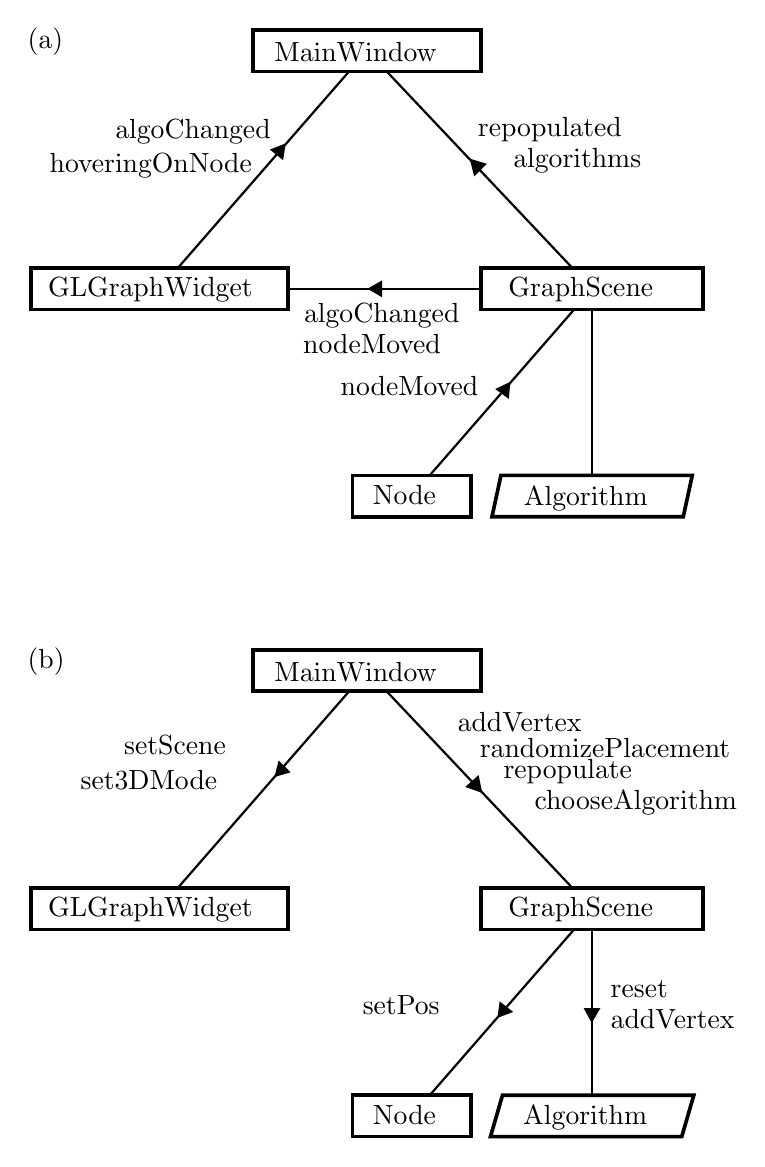
\begin{tikzpicture}[y=0.80pt, x=0.8pt,yscale=-1, inner sep=0pt, outer sep=0pt]
\begin{scope}[shift={(-112.55702,-213.37695)}]
  \begin{scope}[cm={{0.60244614,0.0,0.0,0.60244614,(61.856524,54.195329)}}]
    \path[draw=black,line width=1.328pt,rounded corners=0.0000cm]
      (268.2596,281.6544) rectangle (438.9601,312.6544);
    \path[fill=black] (284.14697,305.60364) node[above right] (text3003) {MainWindow
      };
  \end{scope}
  \begin{scope}[cm={{0.60244614,0.0,0.0,0.60244614,(41.49929,104.70602)}}]
    \path[fill=black] (148.19138,401.63339) node[above right] (text2991)
      {GLGraphWidget       };
    \path[draw=black,line width=1.328pt,rounded corners=0.0000cm]
      (135.3776,376.3655) rectangle (328.3015,407.3655);
  \end{scope}
  \begin{scope}[cm={{0.60244614,0.0,0.0,0.60244614,(88.967165,105.34863)}}]
    \path[fill=black] (414.52719,400.70734) node[above right] (text2995) {GraphScene
      };
    \path[draw=black,line width=1.328pt,rounded corners=0.0000cm]
      (393.9723,375.2989) rectangle (560.6322,406.2989);
  \end{scope}
  \begin{scope}[cm={{0.60244614,0.0,-0.13122252,0.60244614,(154.0838,136.35127)}}]
    \path[fill=black] (428.1041,505.48331) node[above right] (text2987) {Algorithm
      };
    \path[draw=black,line width=1.328pt,rounded corners=0.0000cm]
      (405.2505,479.1763) rectangle (548.6769,510.1763);
  \end{scope}
  \path[draw=black,line join=miter,line cap=butt,line width=0.800pt]
    (189.3056,331.4460) -- (266.7520,242.5528);
  \path[draw=black,line join=miter,line cap=butt,line width=0.800pt]
    (283.7097,242.5528) -- (367.6938,331.4460);
  \path[draw=black,line join=miter,line cap=butt,line width=0.800pt]
    (326.3143,340.7839) -- (239.2832,340.7839);
  \path[draw=black,line join=miter,line cap=butt,line width=0.800pt]
    (376.5161,350.1218) -- (376.5161,425.0292);
  \path[fill=black] (246.43787,358.36713) node[above right] (text3059)
    {algoChanged     };
  \path[fill=black] (246.03421,370.05441) node[above right] (text3063) {nodeMoved
    };
  \path[cm={{0.60244614,0.0,0.0,0.60244614,(219.19954,185.07318)}},draw=black,fill=black,line
    join=miter,line cap=butt,miter limit=4.00,line width=1.328pt]
    (102.3179,254.4263) -- (102.2747,262.3632) -- (95.4227,258.3573) -- cycle;
  \path[cm={{0.59608163,0.08733863,-0.08733863,0.59608163,(198.29375,115.77633)}},draw=black,fill=black,line
    join=miter,line cap=butt,miter limit=4.00,line width=1.328pt]
    (102.3179,254.4263) -- (102.2747,262.3632) -- (95.4227,258.3573) -- cycle;
  \path[cm={{-0.69799145,0.17382972,-0.18444507,-0.71573379,(441.95326,452.94883)}},draw=black,fill=black,line
    join=miter,line cap=butt,miter limit=4.00,line width=1.097pt]
    (102.3179,254.4263) -- (102.2747,262.3632) -- (95.4227,258.3573) -- cycle;
  \path[fill=black] (161.1712,275.12494) node[above right] (text3118) {algoChanged
    };
  \path[fill=black] (131.48926,290.81223) node[above right] (text3122)
    {hoveringOnNode     };
  \begin{scope}[cm={{0.60244614,0.0,0.0,0.60244614,(80.129239,88.883392)}}]
    \path[fill=black] (327.60049,579.53265) node[above right] (text3128) {Node
      };
    \path[draw=black,line width=1.328pt,rounded corners=0.0000cm]
      (312.2591,557.9682) rectangle (401.1372,588.9682);
  \end{scope}
  \path[draw=black,line join=miter,line cap=butt,line width=0.800pt]
    (303.1524,425.0292) -- (368.3843,350.1218);
  \path[cm={{0.58190708,0.05230551,-0.04887953,0.5983474,(291.49485,226.59278)}},draw=black,fill=black,line
    join=miter,line cap=butt,miter limit=4.00,line width=1.351pt]
    (102.3179,254.4263) -- (102.2747,262.3632) -- (95.4227,258.3573) -- cycle;
  \path[fill=black] (262.92914,388.73416) node[above right] (text3146) {nodeMoved
    };
  \path[fill=black] (324.94656,274.44034) node[above right] (text3150)
    {repopulated     };
  \path[fill=black] (121.5652,235.30273) node[above right] (text3889) {(a)     };
  \begin{scope}[cm={{0.60244614,0.0,0.0,0.60244614,(61.856524,334.19533)}}]
    \path[draw=black,line width=1.328pt,rounded corners=0.0000cm]
      (268.2596,281.6544) rectangle (438.9601,312.6544);
    \path[fill=black] (284.14697,305.60364) node[above right] (text3901) {MainWindow
      };
  \end{scope}
  \begin{scope}[cm={{0.60244614,0.0,0.0,0.60244614,(41.49929,384.70602)}}]
    \path[fill=black] (148.19138,401.63339) node[above right] (text3907)
      {GLGraphWidget       };
    \path[draw=black,line width=1.328pt,rounded corners=0.0000cm]
      (135.3776,376.3655) rectangle (328.3015,407.3655);
  \end{scope}
  \begin{scope}[cm={{0.60244614,0.0,0.0,0.60244614,(88.967165,385.34863)}}]
    \path[fill=black] (414.52719,400.70734) node[above right] (text3915) {GraphScene
      };
    \path[draw=black,line width=1.328pt,rounded corners=0.0000cm]
      (393.9723,375.2989) rectangle (560.6322,406.2989);
  \end{scope}
  \begin{scope}[cm={{0.60244614,0.0,-0.17496336,0.60244614,(175.72135,416.35127)}}]
    \path[fill=black] (428.44839,505.48331) node[above right] (text3923) {Algorithm
      };
    \path[draw=black,line width=1.328pt,rounded corners=0.0000cm]
      (405.2505,479.1763) rectangle (548.6769,510.1763);
  \end{scope}
  \path[draw=black,line join=miter,line cap=butt,line width=0.800pt]
    (189.3056,611.4460) -- (266.7520,522.5528);
  \path[draw=black,line join=miter,line cap=butt,line width=0.800pt]
    (283.7097,522.5528) -- (367.6938,611.4460);
  \path[draw=black,line join=miter,line cap=butt,line width=0.800pt]
    (376.5161,630.1218) -- (376.5161,705.0292);
  \path[cm={{-0.58532849,-0.14258998,0.14258998,-0.58532849,(257.79281,723.57069)}},draw=black,fill=black,line
    join=miter,line cap=butt,miter limit=4.00,line width=1.328pt]
    (102.3179,254.4263) -- (102.2747,262.3632) -- (95.4227,258.3573) -- cycle;
  \path[cm={{0.70569892,-0.13927625,0.14900577,0.72394207,(214.68757,391.73552)}},draw=black,fill=black,line
    join=miter,line cap=butt,miter limit=4.00,line width=1.097pt]
    (102.3179,254.4263) -- (102.2747,262.3632) -- (95.4227,258.3573) -- cycle;
  \path[fill=black] (165.1712,551.12494) node[above right] (text3951) {setScene
    };
  \path[fill=black] (145.48926,566.81226) node[above right] (text3955) {set3DMode
    };
  \begin{scope}[cm={{0.60244614,0.0,0.0,0.60244614,(80.129239,368.88339)}}]
    \path[fill=black] (327.60049,579.53265) node[above right] (text3961) {Node
      };
    \path[draw=black,line width=1.328pt,rounded corners=0.0000cm]
      (312.2591,557.9682) rectangle (401.1372,588.9682);
  \end{scope}
  \path[draw=black,line join=miter,line cap=butt,line width=0.800pt]
    (303.1524,705.0292) -- (368.3843,630.1218);
  \path[cm={{0.35985131,-0.46028117,0.47594756,0.3658999,(177.46665,618.17186)}},draw=black,fill=black,line
    join=miter,line cap=butt,miter limit=4.00,line width=1.351pt]
    (102.3179,254.4263) -- (102.2747,262.3632) -- (95.4227,258.3573) -- cycle;
  \path[fill=black] (272.92914,668.73413) node[above right] (text3971) {setPos
    };
  \path[fill=black] (315.80371,540.58319) node[above right] (text3975) {addVertex
    };
  \path[fill=black] (121.5652,515.30273) node[above right] (text3979) {(b)     };
  \path[fill=black] (325.80371,552.58319) node[above right] (text3983)
    {randomizePlacement     };
  \path[fill=black] (336.51801,564.58319) node[above right] (text3987) {repopulate
    };
  \path[fill=black] (340.94656,288.44034) node[above right] (text3991) {algorithms
    };
  \path[fill=black] (350.51801,578.58319) node[above right] (text3995)
    {chooseAlgorithm     };
  \path[cm={{0.50323671,0.29682408,-0.30078027,0.51955755,(403.81881,503.95313)}},draw=black,fill=black,line
    join=miter,line cap=butt,miter limit=4.00,line width=1.351pt]
    (102.3179,254.4263) -- (102.2747,262.3632) -- (95.4227,258.3573) -- cycle;
  \path[fill=black] (384.92914,660.73413) node[above right] (text4001) {reset
    };
  \path[fill=black] (384.92914,674.73413) node[above right] (text4005) {addVertex
    };
\end{scope}

\end{tikzpicture}

  \caption{Flow of (a) information upwards via \code{signal}s and (b)
    commands downward}
  \label{fig:interaction}
\end{figure}

\subsection{Graph drawing}

When writing the renderer, we considered using various graphics
libraries which allow for platform-independent drawing using
primitives. Candidates were \Cairo\footnote{\Cairo homepage:
  \href{http://cairographics.org/}{cairographics.org}}, \Qt and
\OpenGL. The first two are the most common 2D drawing libraries used
in modern open-source software; however, since they operate mostly on
the CPU (with hardware-acceleration being very limited), they proved
too slow for the large graphs we wished to visualise\footnote{during
  our first iteration, we wrote a prototype for each of the libraries
  in order to benchmark their speed and ease of development; \Qt won
  on ease of development, which is what we used for rendering during
  the early iterations; \OpenGL won on speed, which is what we decided
  to use in the end}.

In the end, we decided to use \OpenGL for drawing graphs on the
screen. Thanks to its hardware accelerated nature, Visigoth can
(re-)draw thousands of nodes and edges often enough every second to
give the user the impression of a smooth interface when interacting
with the graph.

Whilst implementing the camera handling, the node/edge drawing and the
interface allowing the user to `fly' through a 3D graph, we developed
a helper library, \code{glAncillary}. A significant portion of our
code can now be reused in similar \OpenGL projects; this is important
since applications such as Visigoth require a completely different
kind of graphics engine than the ones commonly found in other 3D
applications such as video games.

%% FIXME Max, could you say a few words about an issue you encountered
%% and how you fixed it? (for instance, dragging in 3D)


\subsection{Graph layout}
Laying out a graph is a tricky problem, mainly due to the fact that the
prime interest when engineering layouts is to please humans' taste
instead of some logical property. A wide array of such algorithms have
been proposed, and since drawing graphs is a central task in Visigoth,
we had to choose the one that fit best.

First we experimented with the existing solutions. One of the most
complete free graph-drawing algorithm is
GraphViz\footnote{\myhref{www.graphviz.org}},
and it provides various algorithms:

\begin{description}
\item [dot] A hierarchical layout, used for directed graphs. Our small
  world networks are not directed and it was clear from the beginning
  that they did not fit this model well.

\item [twopi, circo] Radial and circular layout, respectively. Again,
  unsuitable for the quasi-random networks that we use in Visigoth.

\item [neato] A spring model layout, which seemed to work reasonably
  well with random graphs.
\end{description}

The spring model seemed to be the best fit. This class of algorithm
work by treating edges like springs: in this way clusters of highly
connected nodes would be drawn together. To counter this force (that
would lead to nodes lumping together), nodes are treated as charged
particles of the same polarity, causing repulsion between every node
and the others.

When generating a graph, the nodes are first places at random
locations in the space. Then, we apply the algorithm repeatedly until
the forces are low enough that we can consider the graph to be stable.

Spring model algorithms are nice for two reasons:

\begin{itemize}
\item Good results: spring force algorithms produce pleasant graphs
  for almost all kind of networks. Some algorithms might produce
  better results for specific kinds of graph, but spring force
  algorithms are by far the more adaptive.

\item Ease of implementation: Our simple implementation of the
  algorithm take a little less then 50 lines of \buzz{C++} code, and
  works well up to medium-sized graphs.

\item Real time drawing: force based algorithms can be used to show in
  real time the untangling of the graph, which is usually an
  interesting effect. It also permits interaction, for example in the
  form of node-dragging that changes the shape of the graph. We employ
  both techniques in Visigoth.
\end{itemize}

\subsubsection{FADE}

However, even a simple description of the algorithms reveals its high
cost. For each particle, we need to iterate through all the connected
nodes to calculate the spring forces, and more importantly through all
the particles of the graphs to calculate the repulsion forces. Thus,
the algorithm is \(O(n^2)\), where \(n\) is the number of nodes.

For this reason, our implementation works smoothly up to around a
\(1000\) nodes, but then performance degrades quickly, and the program
becomes unresponsive. Various solutions have been studied, most of
which rely on various approximations.

We chose to implement the \emph{FADE} algorithm \cite{fade}, which works by
recursively subdividing the graph space into sub-spaces, and then
treats sub-spaces as single particles when they are far enough. This
algorithm, while improving performance, is a lot more complex then the
naive one.

\begin{figure}[ht!]
  \centering
  \subfloat[Graph view]{
    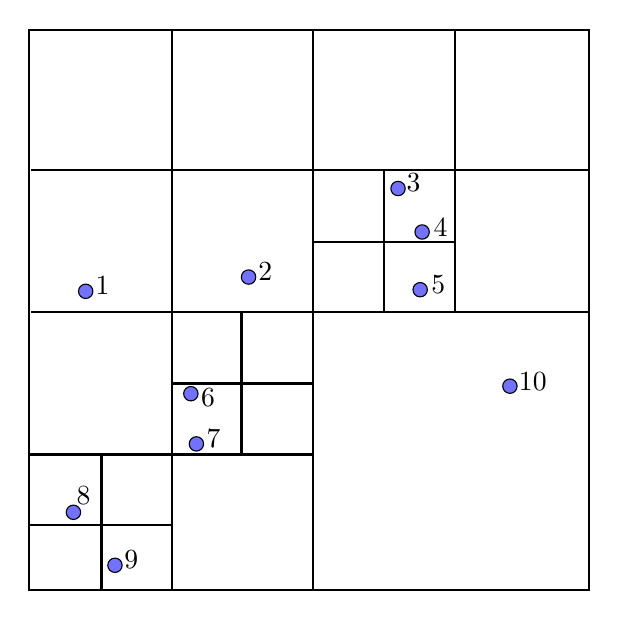
\begin{tikzpicture}[y=0.80pt, x=0.8pt,yscale=-0.5, xscale=0.5, inner sep=0pt, outer sep=0pt]
  \path[draw=black,line join=miter,line cap=butt,line width=0.800pt]
  (356.4286,94.5050) -- (356.4286,598.7908);
  \path[draw=black,line join=miter,line cap=butt,line width=0.800pt]
  (102.1429,348.7908) -- (605.7143,348.7908);
  \path[draw=black,line join=miter,line cap=butt,line width=0.800pt]
  (102.1429,220.2193) -- (607.1429,220.2193);
  \path[draw=black,line join=miter,line cap=butt,line width=0.800pt]
  (229.2857,93.0765) -- (229.2857,598.7908);
  \path[draw=black,line join=miter,line cap=butt,line width=0.800pt]
  (485.0000,93.7908) -- (485.0000,349.5050);
  \path[draw=black,line join=miter,line cap=butt,line width=0.800pt]
  (101.4286,477.3622) -- (356.4286,477.3622);
  \path[draw=black,line join=miter,line cap=butt,line width=0.800pt]
  (420.7143,220.2193) -- (420.7143,349.5050);
  \path[draw=black,line join=miter,line cap=butt,line width=0.800pt]
  (356.4286,285.2193) -- (485.0000,285.2193);
  \path[draw=black,line join=miter,line cap=butt,line width=0.800pt]
  (292.1429,348.0765) -- (292.1429,476.6479);
  \path[draw=black,line join=miter,line cap=butt,line width=0.800pt]
  (228.5714,413.0765) -- (357.1429,413.0765);
  \path[draw=black,line join=miter,line cap=butt,line width=0.800pt]
  (165.7143,477.3622) -- (165.7143,599.5050);
  \path[draw=black,line join=miter,line cap=butt,line width=0.800pt]
  (100.7143,540.9336) -- (229.2857,540.9336);
  \path[cm={{0.86607143,0.0,0.0,0.86607143,(-133.53636,-75.700851)}},draw=black,fill=c7372ff]
  (506.4286,453.4336)arc(0.000:180.000:7.500)arc(-180.000:0.000:7.500) -- cycle;
  \path[cm={{0.86607143,0.0,0.0,0.86607143,(-280.6792,-62.843726)}},draw=black,fill=c7372ff]
  (506.4286,453.4336)arc(0.000:180.000:7.500)arc(-180.000:0.000:7.500) -- cycle;
  \path[cm={{0.86607143,0.0,0.0,0.86607143,(-185.6792,29.656274)}},draw=black,fill=c7372ff]
  (506.4286,453.4336)arc(0.000:180.000:7.500)arc(-180.000:0.000:7.500) -- cycle;
  \path[cm={{0.86607143,0.0,0.0,0.86607143,(-180.6792,75.013418)}},draw=black,fill=c7372ff]
  (506.4286,453.4336)arc(0.000:180.000:7.500)arc(-180.000:0.000:7.500) -- cycle;
  \path[cm={{0.86607143,0.0,0.0,0.86607143,(-291.75062,136.79913)}},draw=black,fill=c7372ff]
  (506.4286,453.4336)arc(0.000:180.000:7.500)arc(-180.000:0.000:7.500) -- cycle;
  \path[cm={{0.86607143,0.0,0.0,0.86607143,(-254.25063,184.65628)}},draw=black,fill=c7372ff]
  (506.4286,453.4336)arc(0.000:180.000:7.500)arc(-180.000:0.000:7.500) -- cycle;
  \path[cm={{0.86607143,0.0,0.0,0.86607143,(102.53509,22.87056)}},draw=black,fill=c7372ff]
  (506.4286,453.4336)arc(0.000:180.000:7.500)arc(-180.000:0.000:7.500) -- cycle;
  \path[cm={{0.86607143,0.0,0.0,0.86607143,(21.463659,-64.272297)}},draw=black,fill=c7372ff]
  (506.4286,453.4336)arc(0.000:180.000:7.500)arc(-180.000:0.000:7.500) -- cycle;
  \path[cm={{0.86607143,0.0,0.0,0.86607143,(23.249374,-116.41515)}},draw=black,fill=c7372ff]
  (506.4286,453.4336)arc(0.000:180.000:7.500)arc(-180.000:0.000:7.500) -- cycle;
  \path[cm={{0.86607143,0.0,0.0,0.86607143,(1.4636592,-155.70087)}},draw=black,fill=c7372ff]
  (506.4286,453.4336)arc(0.000:180.000:7.500)arc(-180.000:0.000:7.500) -- cycle;
  \path[fill=black] (160.31509,332.78058) node[above right] (text6462) {1};
  \path[fill=black] (307.43341,319.70856) node[above right] (text6462-4) {2};
  \path[fill=black] (441.40405,239.94313) node[above right] (text6462-9) {3};
  \path[fill=black] (465.61832,280.30029) node[above right] (text6462-98) {4};
  \path[fill=black] (463.73944,332.14725) node[above right] (text6462-5) {5};
  \path[fill=black] (255.68974,433.98373) node[above right] (text6462-0) {6};
  \path[fill=black] (260.68976,470.65741) node[above right] (text6462-7) {7};
  \path[fill=black] (143.21951,522.34161) node[above right] (text6462-3) {8};
  \path[fill=black] (186.40405,580.65741) node[above right] (text6462-43) {9};
  \path[fill=black] (542.83264,419.586) node[above right] (text6462-02) {10};
  \path[draw=black,line join=miter,line cap=butt,line width=0.800pt]
  (606.0915,92.7173) -- (606.0915,599.8138) -- (100.0051,599.8138) --
  (100.0051,92.7173);
  \path[draw=black,line join=miter,line cap=butt,line width=0.800pt]
  (100.0051,93.7274) -- (605.0814,93.7274);
\end{tikzpicture}

  }
  \hspace{4pt}
  \subfloat[Tree representation]{
    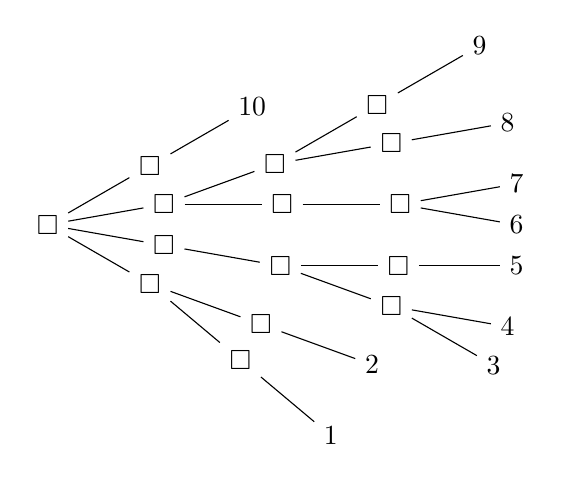
\begin{tikzpicture}[grow cyclic]
  \node {\square}
  child {
    node {\square}
    child {
      node {\square}
      child {node {1}}
    }
    child {
      node {\square}
      child {node {2}}
    }
  }
  child {
    node {\square}
    child {
      node {\square}
      child {
        node {\square}
        child { node{3} }
        child { node{4} }
      }
      child {
        node {\square}
        child {node{5}}
      }
    }
  }
  child {
    node {\square}
    child {
      node {\square}
      child {
        node {\square}
        child {node{6}}
        child {node{7}}
      }
    }
    child {
      node {\square}
      child {
        node {\square}
        child {node{8}}
      }
      child {
        node {\square}
        child {node{9}}
      }
    }
  }
  child {
    node {\square}
    child { node {10} }
  }
  ;
\end{tikzpicture}

  }
  \caption{The QuadTree for a sample graph, empty branches omitted}
  \label{fig:quadtree}
\end{figure}

The first step is to build a data structure representing the recursive
subdivision. This kind of data structure is called a \emph{TreeCode},
which recursively subdivides the space until only one node remains in
the current space, or a maximum depth/minimum space size size is
hit. The space decomposition can be irregular (e.g. \emph{Voronoi}
spaces) or regular. In the latter case, the space is recursively
subdivided in squares. We chose to use a regular, 4-way space
decomposition, mainly due to its simplicity. This kind of structure is
called \emph{QuadTree}. Figure \ref{fig:quadtree} shows a sample
QuadTree for a Visigoth graph. In the QuadTree, each sub-quadrant
preserved the weighted centre of gravity relative to the contained
nodes.

Building the tree is the difficult part of the algorithm and can be
done in linear time. Once that is done, to calculate the non-edge
forces for a given node the algorithm proceeds as indicated in figure
\ref{proc:FADE}.

\begin{figure}[ht!]
  \begin{minipage}[b]{0.5\linewidth}
    \begin{algorithmic}
  \REQUIRE \(0 < \theta < 1\)
  \REQUIRE \(\beta > 1\)
  \REQUIRE \(\vec{n} \neq \vec{q}\)
\end{algorithmic}
force\((n, q)\):
\begin{algorithmic}
  \STATE \(\vec{d} \gets \vec{n} - \vec{q}\)
  \IF { \(q\) is terminal \OR \(\frac{\vec{d}}{\textrm{width}(q)} < \theta\) }
  \STATE \(\vec{v} \gets \vec{d} \cdot \frac{\beta}{|{\vec{d}}|^2}\)
  \STATE \(\vec{v} \gets \vec{v} \cdot \textrm{mass}(q)\)
  \RETURN \(\vec{v} \cdot \frac{\beta}{|{\vec{d}}|^2}\)
  \ELSE
  \STATE \(\vec{v} \gets 0\)
  \FOR {\(q'\) in children\((q)\)}
  \STATE \(\vec{v} \gets \vec{v} + \textrm{force}(n, q')\)
  \ENDFOR
  \RETURN \(\vec{v}\)
  \ENDIF
\end{algorithmic}

    \caption{This procedure calculates the non-edge force of a given
      node \(n\), given the QuadTree \(q\). \(\vec{n}\) and
      \(\vec{q}\) indicate the vectors corresponding to the respective
      centers of gravity. \(\beta\) is an empirically determined
      parameter used to regulate the amount of force - \(75\) has
      worked well for us. \(\theta\) is central to the FADE algorithm
      and determines the amount of approximation. If \(\geq 1\) the
      algorithm is unstable, we used values between \(0.5\) and
      \(0.8\). See figure \ref{fig:theta} for a visual
      explanation. The mass of a quadrant is simply the number of
      nodes residing in it. }
    \label{proc:FADE}
  \end{minipage}
  \hspace{10pt}
  \begin{minipage}[b]{0.5\linewidth}
    \centering
    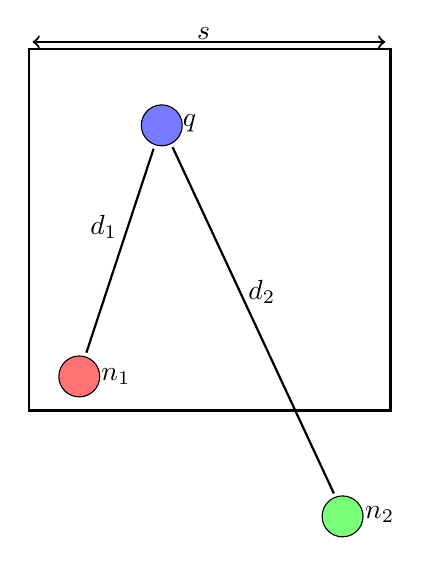
\begin{tikzpicture}[y=0.80pt, x=0.8pt,yscale=-1, inner sep=0pt, outer sep=0pt]
  \path[draw=black,fill=cffffff,line join=miter,line cap=butt,fill
    opacity=0.000,even odd rule,line width=0.803pt,rounded corners=0.0000cm]
  (140.4134,176.5621) rectangle (303.7579,339.9066);
  \path[cm={{0.79503474,0.0,0.0,0.79503474,(-296.23722,-12.403676)}},draw=black,fill=c787aff]
  (636.3961,281.1107)arc(0.000:180.000:11.617)arc(-180.000:0.000:11.617) --
  cycle;
  \path[cm={{0.79503474,0.0,0.0,0.79503474,(-333.50701,101.01225)}},draw=black,fill=cff7374]
  (636.3961,281.1107)arc(0.000:180.000:11.617)arc(-180.000:0.000:11.617) --
  cycle;
  \path[cm={{0.79503474,0.0,0.0,0.79503474,(-214.57843,164.22654)}},draw=black,fill=c79ff79]
  (636.3961,281.1107)arc(0.000:180.000:11.617)arc(-180.000:0.000:11.617) --
  cycle;
  \path[draw=black,line join=miter,line cap=butt,line width=0.800pt]
  (166.4286,313.7908) -- (196.7857,221.6479);
  \path[draw=black,line join=miter,line cap=butt,line width=0.800pt]
  (205.3571,220.9336) -- (278.2143,377.3622);
  \path[fill=black] (168.21428,262.36218) node[above right] (text5235) {\(d_1\)};
  \path[fill=black] (239.64287,291.64789) node[above right] (text5239) {\(d_2\)};
  \path[fill=black] (216.42857,172.36218) node[above right] (text5243) {\(s\)};
  \path (142.5000,173.7908) -- (300.0000,173.7908);
  \path[draw=black,line join=miter,line cap=butt,line width=0.800pt, <->]
  (142.1429,173.4336) -- (301.4286,173.4336);
  \path[fill=black] (210,214.1479) node[above right] (text5479) {\(q\)};
  \path[fill=black] (173.21429,328.07648) node[above right] (text5483) {\(n_1\)};
  \path[fill=black] (292.34625,390.3728) node[above right] (text5483-5) {\(n_2\)};
\end{tikzpicture}

    \caption{In this case, \(n_1\) and \(n_2\) are nodes and \(q\) is
      a quadrant with edge length \(s\). When calculating the non-edge
      force between \(n_1\) and \(q\), where \(s\) is the quadrant
      will be judged to be too close to approximate, since
      \(\frac{s}{d_1} > 1\), while \(n_2\) might be judged far enough,
      depending on \(\theta\).}
    \label{fig:theta}
  \end{minipage}
\end{figure}

Once implemented, the FADE algorithm lead to great speedups while
preserving good node placements. While drawing \(1000\) nodes is
already difficult with the simple algorithm, FADE can easily handle
\(10000\) nodes, after which other performance limits are hit (the
graph generation time and the \OpenGL drawing).

After we implemented the 3D view we had to write an extension to FADE to support
3D, which proved to be straight forward. Now we have a 3-dimensional space,
which is recursively divided into $8$ cubes.

\subsection{Effort}

Work was divided between team members such that each would focus on
developing a particular component and reviewing another. Table
\ref{fig:effort} gives an overview of the distribution of work and the
amount of effort required to finish each component.

\begin{figure}[ht!]
  \centering
  \begin{tabular}{c|c|c}
    Component         & Team members    & Effort \\
    \hline
    GUI               & Ingrid, Max     & ~80 phrs \\
    3D Renderer       & Max, Francesco  & ~60 phrs\\
    \code{GraphScene} & Francesco, Alex & ~80 phrs\\
    Algorithms        & Marc, Ingrid    & ~120 phrs\\
    Testing           & Alex, Marc      & ~20 phrs\\
    \hline
    Total             &                 & ~360 phrs
  \end{tabular}
  \caption{Effort expanded on each component in person-hours}
  \label{fig:effort}
\end{figure}

An \emph{impact} graph, as generated by
\GitHub\footnote{\href{https://github.com}{github.com}} is included in Figure
\ref{fig:impact}. It shows that, at least in terms of
SLOC\footnote{\myhref{en.wikipedia.org/wiki/Source\_lines\_of\_code}},
the effort was well spread out across the development team.

\begin{figure}[ht!]
  \centering
  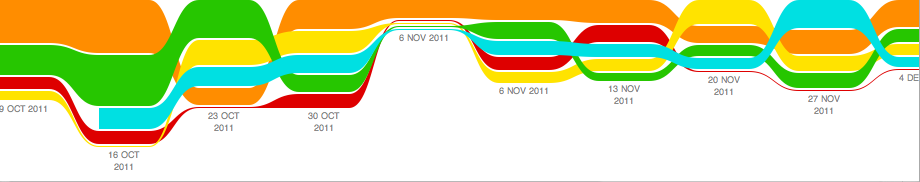
\includegraphics[width=\textwidth]{impact.png}
  \caption{Development impact of team members}
  \label{fig:impact}
\end{figure}

The total amount of code\footnote{as generated using David
  A. Wheeler's `SLOCCount'} required for each component is included in
Figure \ref{fig:sloc}. Note that this table does not show the all the
code that did \emph{not} make it into the final product; for instance,
the renderer went through two complete rewrites before being the
current 3D Renderer.

\begin{figure}[ht!]
  \centering
  \begin{tabular}{c|l}
    Component         & SLOC \\
    \hline
    GUI               & $180$ \buzz{C++}, 1037 \buzz{XML}\\
    3D Renderer       & $452$ \buzz{C++}, 82 \buzz{C}\\
    \code{GraphScene} & $686$ \buzz{C++}\\
    Algorithms        & $1220$ \buzz{C++}\\
    Testing           & $238$ \buzz{C++} \\
    \hline
    Total             & $3061$ \buzz{C++}, $1037$ \buzz{XML}, $82$ \buzz{C}
  \end{tabular}
  \caption{Lines of code in each component}
  \label{fig:sloc}
\end{figure}

\subsection{Development practices}
\label{practices}

\subsubsection{Iterative development}

We chose an iterative development model, where each iteration
consisted of adding a small number of features to the existing
product.  Figure \ref{fig:iterations} represents the original
schedule, to which we have adhered until the end.

\begin{figure}[ht!]
  \centering
  
\definecolor{ccfe2f3}{RGB}{207,226,243}
\definecolor{cff9900}{RGB}{255,153,0}
\definecolor{cffff00}{RGB}{255,255,0}

\begin{tikzpicture}[y=0.80pt, x=0.8pt,yscale=-1, inner sep=0pt, outer sep=0pt,
miter limit=10.00]
\path[draw,fill=ccfe2f3,nonzero rule] (320.3063,28.4017) -- (413.1141,28.4017)
  -- (413.1141,145.6695) -- (320.3063,145.6695) -- cycle;
\begin{scope}[cm={{0.76902767,0.0,0.0,0.76801007,(3.762955,1.2016597)}}]
  \path[draw=black,line join=round,line cap=butt,miter limit=10.00,line
    width=1.041pt] (411.7821,36.0097) -- (532.4642,36.0097) -- (532.4642,188.4502)
    -- (411.7821,188.4502) -- cycle;
  \path[draw=black,line join=round,line cap=butt,miter limit=10.00,line
    width=1.041pt] (411.7821,150.3401) -- (532.4642,150.3401);
  \path[draw=black,line join=round,line cap=butt,miter limit=10.00,line
    width=1.041pt] (443.4227,35.8801) -- (443.4227,150.2105);
  \path[draw=black,line join=round,line cap=butt,miter limit=10.00,line
    width=1.041pt] (500.4465,35.7387) -- (500.4465,150.0691);
\end{scope}
\path[draw,fill=ccfe2f3,nonzero rule] (149.3445,116.4041) -- (149.3445,28.5012)
  -- (193.3061,116.4041) -- cycle;
\path[draw,fill=ccfe2f3,nonzero rule] (222.6138,28.4017) -- (315.5755,28.4017)
  -- (315.5755,145.4198) -- (222.6138,145.4198) -- cycle;
\begin{scope}[cm={{0.76902767,0.0,0.0,0.76801007,(3.762955,1.2016597)}}]
  \path[draw=black,line join=round,line cap=butt,miter limit=10.00,line
    width=1.041pt] (284.7484,36.0097) -- (405.4304,36.0097) -- (405.4304,188.4502)
    -- (284.7484,188.4502) -- cycle;
  \path[draw=black,line join=round,line cap=butt,miter limit=10.00,line
    width=1.041pt] (284.7484,150.3401) -- (405.4304,150.3401);
  \path[draw=black,line join=round,line cap=butt,miter limit=10.00,line
    width=1.041pt] (316.3890,35.8801) -- (316.3890,150.2105);
  \path[draw=black,line join=round,line cap=butt,miter limit=10.00,line
    width=1.041pt] (373.4128,35.7387) -- (373.4128,150.0691);
\end{scope}
\path[draw,fill=ccfe2f3,nonzero rule] (193.2336,116.2091) -- (193.2336,28.7863)
  -- (217.4452,116.2091) -- cycle;
\path[draw,fill=ccfe2f3,nonzero rule] (125.1797,28.8134) -- (149.3143,28.8134)
  -- (149.3143,116.4282) -- (125.1797,116.4282) -- cycle;
\begin{scope}[cm={{0.76902767,0.0,0.0,0.76801007,(3.762955,1.2016597)}}]
  \path[draw=black,line join=round,line cap=butt,miter limit=10.00,line
    width=1.041pt] (157.7147,36.0097) -- (278.3968,36.0097) -- (278.3968,188.4502)
    -- (157.7147,188.4502) -- cycle;
  \path[draw=black,line join=round,line cap=butt,miter limit=10.00,line
    width=1.041pt] (157.7147,150.3401) -- (278.3968,150.3401);
  \path[draw=black,line join=round,line cap=butt,miter limit=10.00,line
    width=1.041pt] (189.3553,35.8801) -- (189.3553,150.2105);
  \path[draw=black,line join=round,line cap=butt,miter limit=10.00,line
    width=1.041pt] (246.3791,35.7387) -- (246.3791,150.0691);
\end{scope}
\path[xscale=1.001,yscale=0.999,fill=black] (199.26541,78.484428) node[above
  right] (text5055) {UI   };
\path[draw,fill=ccfe2f3,nonzero rule] (125.0890,145.3284) -- (125.0890,116.2900)
  -- (217.6084,145.3284) -- cycle;
\path[draw,fill=ccfe2f3,nonzero rule] (27.5053,116.4265) -- (27.5053,28.3700) --
  (51.8515,116.4265) -- cycle;
\begin{scope}[cm={{0.76902767,0.0,0.0,0.76801007,(3.762955,1.2016597)}}]
  \path[draw=black,line join=round,line cap=butt,miter limit=10.00,line
    width=1.041pt] (30.5138,35.6754) -- (151.1959,35.6754) -- (151.1959,188.1159)
    -- (30.5138,188.1159) -- cycle;
  \path[draw=black,line join=round,line cap=butt,miter limit=10.00,line
    width=1.041pt] (30.5138,150.0058) -- (151.1959,150.0058);
  \path[draw=black,line join=round,line cap=butt,miter limit=10.00,line
    width=1.041pt] (62.1544,35.5458) -- (62.1544,149.8762);
  \path[draw=black,line join=round,line cap=butt,miter limit=10.00,line
    width=1.041pt] (119.1782,35.4044) -- (119.1782,149.7348);
\end{scope}
\path[draw=black,fill,line join=round,line cap=butt,line width=1.600pt]
  (27.1111,165.3748) -- (27.1111,153.1794);
\path[draw=black,fill=black,line cap=butt,miter limit=10.00,even odd rule,line
  width=0.800pt] (29.1282,153.1794) -- (27.1111,147.6450) -- (25.0941,153.1794)
  -- cycle;
\path[draw=black,fill,line join=round,line cap=butt,line width=1.600pt]
  (121.8628,165.3748) -- (121.8628,153.1794);
\path[draw=black,fill=black,line cap=butt,miter limit=10.00,even odd rule,line
  width=0.800pt] (123.8799,153.1794) -- (121.8628,147.6450) --
  (119.8458,153.1794) -- cycle;
\path[draw=black,fill,line join=round,line cap=butt,line width=1.600pt]
  (220.1761,164.7638) -- (220.1761,152.5684);
\path[draw=black,fill=black,line cap=butt,miter limit=10.00,even odd rule,line
  width=0.800pt] (222.1931,152.5684) -- (220.1761,147.0341) --
  (218.1590,152.5684) -- cycle;
\path[draw=black,fill,line join=round,line cap=butt,line width=1.600pt]
  (318.4712,165.1892) -- (318.4712,152.9938);
\path[draw=black,fill=black,line cap=butt,miter limit=10.00,even odd rule,line
  width=0.800pt] (320.4882,152.9938) -- (318.4712,147.4594) --
  (316.4541,152.9938) -- cycle;
\path[draw=black,fill,line join=round,line cap=butt,line width=1.600pt]
  (413.1141,165.1892) -- (413.1141,152.9938);
\path[draw=black,fill=black,line cap=butt,miter limit=10.00,even odd rule,line
  width=0.800pt] (415.1311,152.9938) -- (413.1141,147.4594) --
  (411.0971,152.9938) -- cycle;
\path[xscale=1.001,yscale=0.999,fill=black] (45.406025,134.43877) node[above
  right] (text5003) {Algorithms   };
\path[xscale=1.001,yscale=0.999,fill=black] (143.77643,134.43877) node[above
  right] (text5007) {Algorithms   };
\path[xscale=1.001,yscale=0.999,fill=black] (240.60979,134.43877) node[above
  right] (text5011) {Algorithms   };
\path[xscale=1.001,yscale=0.999,fill=black] (337.44312,134.43877) node[above
  right] (text5015) {Algorithms   };
\path[xscale=1.001,yscale=0.999,fill=black] (31.728308,78.484428) node[above
  right] (text5019) {2D   };
\path[xscale=1.001,yscale=0.999,fill=black] (130.13319,78.484428) node[above
  right] (text5023) {2D   };
\path[xscale=1.001,yscale=0.999,fill=black] (226.96655,78.484428) node[above
  right] (text5027) {2D   };
\path[xscale=1.001,yscale=0.999,fill=black] (324.71521,78.484428) node[above
  right] (text5031) {2D   };
\path[xscale=1.001,yscale=0.999,fill=black] (66.130356,78.484428) node[above
  right] (text5035) {3D   };
\path[xscale=1.001,yscale=0.999,fill=black] (164.50076,78.484428) node[above
  right] (text5039) {3D   };
\path[xscale=1.001,yscale=0.999,fill=black] (261.33411,78.484428) node[above
  right] (text5043) {3D   };
\path[xscale=1.001,yscale=0.999,fill=black] (358.16748,78.484428) node[above
  right] (text5047) {3D   };
\path[xscale=1.001,yscale=0.999,fill=black] (100.895,78.484428) node[above
  right] (text5051) {UI   };
\path[xscale=1.001,yscale=0.999,fill=black] (297.6358,78.484428) node[above
  right] (text5059) {UI   };
\path[xscale=1.001,yscale=0.999,fill=black] (394.46915,78.484428) node[above
  right] (text5063) {UI   };
\path[xscale=1.001,yscale=0.999,fill=black] (41.43425,18.799803) node[above
  right] (text5079) {I. Prototype   };
\path[xscale=1.001,yscale=0.999,fill=black] (157.04016,18.799803) node[above
  right] (text5083) {II. 2D   };
\path[xscale=1.001,yscale=0.999,fill=black] (252.3365,18.799803) node[above
  right] (text5087) {III. 3D   };
\path[xscale=1.001,yscale=0.999,fill=black] (326.11429,18.799803) node[above
  right] (text5091) {IV. Stabilisation   };
\path[draw=cff9900,fill=cffff00,line join=round,line cap=butt,nonzero rule,line
  width=1.600pt] (398.5463,33.3032) -- (402.3039,31.4071) -- (399.0457,28.2902)
  -- (403.0464,27.7442) -- (400.5096,23.6189) -- (404.4810,24.4601) --
  (402.8383,19.6075) -- (406.5097,21.7786) -- (405.8733,16.5295) --
  (408.9944,19.8825) -- (409.4075,14.5946) -- (411.7656,18.9011) --
  (413.2002,13.9346) -- (414.6348,18.9011) -- (416.9929,14.5946) --
  (417.4060,19.8825) -- (420.5271,16.5295) -- (419.8907,21.7786) --
  (423.5621,19.6075) -- (421.9194,24.4601) -- (425.8908,23.6189) --
  (423.3540,27.7442) -- (427.3548,28.2902) -- (424.0965,31.4071) --
  (427.8541,33.3032) -- (424.0965,35.1993) -- (427.3548,38.3162) --
  (423.3540,38.8622) -- (425.8908,42.9875) -- (421.9194,42.1463) --
  (423.5621,46.9989) -- (419.8907,44.8278) -- (420.5271,50.0769) --
  (417.4060,46.7239) -- (416.9929,52.0118) -- (414.6348,47.7053) --
  (413.2002,52.6718) -- (411.7656,47.7053) -- (409.4075,52.0118) --
  (408.9944,46.7239) -- (405.8733,50.0769) -- (406.5097,44.8278) --
  (402.8383,46.9989) -- (404.4810,42.1463) -- (400.5096,42.9875) --
  (403.0464,38.8622) -- (399.0457,38.3162) -- (402.3039,35.1993) -- cycle;
\path[draw,fill=black,nonzero rule] (403.5238,28.8955) -- (407.0847,24.4685) --
  (408.7580,25.8113) .. controls (409.0505,26.0461) and (409.2617,26.2400) ..
  (409.3915,26.3930) .. controls (409.5817,26.6027) and (409.7104,26.8180) ..
  (409.7775,27.0389) .. controls (409.8446,27.2598) and (409.8491,27.4976) ..
  (409.7910,27.7525) .. controls (409.7329,28.0073) and (409.6142,28.2461) ..
  (409.4349,28.4690) .. controls (409.1322,28.8453) and (408.7561,29.0670) ..
  (408.3065,29.1340) .. controls (407.8569,29.2010) and (407.3198,28.9839) ..
  (406.6951,28.4826) -- (405.5573,27.5695) -- (404.1114,29.3670) --
  (403.5238,28.8955) -- cycle(405.9754,27.0495) -- (407.1207,27.9686) ..
  controls (407.4975,28.2710) and (407.8232,28.4162) .. (408.0978,28.4044) ..
  controls (408.3725,28.3926) and (408.6134,28.2579) .. (408.8205,28.0004) ..
  controls (408.9679,27.8172) and (409.0473,27.6222) .. (409.0587,27.4154) ..
  controls (409.0701,27.2085) and (409.0168,27.0212) .. (408.8989,26.8533) ..
  controls (408.8196,26.7489) and (408.6462,26.5894) .. (408.3784,26.3745) --
  (407.2480,25.4674) -- (405.9754,27.0495) -- cycle(408.7777,30.4717) ..
  controls (409.2557,29.8775) and (409.7718,29.5705) .. (410.3261,29.5509) ..
  controls (410.7949,29.5360) and (411.2277,29.6877) .. (411.6243,30.0060) ..
  controls (412.0655,30.3601) and (412.3107,30.7931) .. (412.3598,31.3051) ..
  controls (412.4089,31.8171) and (412.2283,32.3282) .. (411.8180,32.8382) ..
  controls (411.4874,33.2492) and (411.1645,33.5238) .. (410.8494,33.6621) ..
  controls (410.5343,33.8003) and (410.2049,33.8395) .. (409.8614,33.7798) ..
  controls (409.5179,33.7200) and (409.2073,33.5787) .. (408.9296,33.3559) ..
  controls (408.4785,32.9939) and (408.2309,32.5588) .. (408.1867,32.0508) ..
  controls (408.1426,31.5428) and (408.3396,31.0164) .. (408.7777,30.4717) --
  cycle(409.3355,30.9193) .. controls (409.0049,31.3303) and (408.8462,31.7102)
  .. (408.8594,32.0589) .. controls (408.8726,32.4077) and (409.0155,32.6914) ..
  (409.2882,32.9103) .. controls (409.5559,33.1251) and (409.8629,33.2024) ..
  (410.2091,33.1421) .. controls (410.5554,33.0818) and (410.8978,32.8412) ..
  (411.2364,32.4203) .. controls (411.5550,32.0242) and (411.7065,31.6507) ..
  (411.6908,31.3000) .. controls (411.6752,30.9493) and (411.5335,30.6665) ..
  (411.2658,30.4517) .. controls (410.9931,30.2328) and (410.6858,30.1533) ..
  (410.3441,30.2131) .. controls (410.0023,30.2729) and (409.6661,30.5083) ..
  (409.3355,30.9193) -- cycle(411.2011,35.0565) -- (414.7620,30.6295) --
  (415.3049,31.0652) -- (411.7440,35.4922) -- (411.2011,35.0565) --
  cycle(415.6784,32.4038) -- (416.1863,31.7725) -- (416.7291,32.2081) --
  (416.2213,32.8395) -- (415.6784,32.4038) -- cycle(412.6253,36.1995) --
  (415.2004,32.9981) -- (415.7433,33.4337) -- (413.1682,36.6351) --
  (412.6253,36.1995) -- cycle(414.5897,36.1992) -- (415.1909,36.5472) ..
  controls (415.0494,36.7840) and (415.0012,37.0163) .. (415.0464,37.2440) ..
  controls (415.0916,37.4718) and (415.2382,37.6852) .. (415.4861,37.8841) ..
  controls (415.7340,38.0830) and (415.9595,38.1805) .. (416.1626,38.1764) ..
  controls (416.3657,38.1724) and (416.5230,38.1010) .. (416.6346,37.9624) ..
  controls (416.7342,37.8386) and (416.7573,37.6983) .. (416.7040,37.5414) ..
  controls (416.6694,37.4322) and (416.5333,37.2211) .. (416.2956,36.9081) ..
  controls (415.9786,36.4908) and (415.7732,36.1833) .. (415.6792,35.9857) ..
  controls (415.5853,35.7881) and (415.5504,35.5931) .. (415.5746,35.4007) ..
  controls (415.5988,35.2083) and (415.6747,35.0328) .. (415.8022,34.8744) ..
  controls (415.9177,34.7308) and (416.0565,34.6242) .. (416.2185,34.5546) ..
  controls (416.3805,34.4850) and (416.5504,34.4563) .. (416.7282,34.4686) ..
  controls (416.8643,34.4718) and (417.0224,34.5111) .. (417.2025,34.5864) ..
  controls (417.3826,34.6617) and (417.5569,34.7670) .. (417.7255,34.9022) ..
  controls (417.9734,35.1012) and (418.1639,35.3131) .. (418.2970,35.5381) ..
  controls (418.4301,35.7631) and (418.4928,35.9743) .. (418.4849,36.1717) ..
  controls (418.4770,36.3691) and (418.4068,36.5857) .. (418.2742,36.8215) --
  (417.6791,36.4661) .. controls (417.7897,36.2778) and (417.8248,36.0922) ..
  (417.7845,35.9090) .. controls (417.7442,35.7259) and (417.6174,35.5488) ..
  (417.4042,35.3777) .. controls (417.1563,35.1788) and (416.9450,35.0764) ..
  (416.7702,35.0706) .. controls (416.5954,35.0648) and (416.4622,35.1188) ..
  (416.3705,35.2327) .. controls (416.3148,35.3020) and (416.2873,35.3818) ..
  (416.2881,35.4721) .. controls (416.2848,35.5673) and (416.3144,35.6726) ..
  (416.3768,35.7878) .. controls (416.4154,35.8513) and (416.5407,36.0252) ..
  (416.7527,36.3094) .. controls (417.0558,36.7237) and (417.2570,37.0237) ..
  (417.3564,37.2095) .. controls (417.4559,37.3952) and (417.4982,37.5860) ..
  (417.4834,37.7819) .. controls (417.4686,37.9778) and (417.3875,38.1674) ..
  (417.2401,38.3506) .. controls (417.0927,38.5338) and (416.9020,38.6619) ..
  (416.6680,38.7348) .. controls (416.4339,38.8077) and (416.1819,38.8091) ..
  (415.9119,38.7391) .. controls (415.6419,38.6691) and (415.3804,38.5326) ..
  (415.1276,38.3297) .. controls (414.7111,37.9955) and (414.4635,37.6542) ..
  (414.3848,37.3058) .. controls (414.3060,36.9575) and (414.3743,36.5886) ..
  (414.5897,36.1991) -- cycle(417.2064,39.8758) -- (420.7674,35.4488) --
  (421.3102,35.8845) -- (420.0317,37.4740) .. controls (420.5195,37.3848) and
  (420.9568,37.4953) .. (421.3435,37.8057) .. controls (421.5815,37.9966) and
  (421.7507,38.2098) .. (421.8510,38.4451) .. controls (421.9513,38.6804) and
  (421.9729,38.9096) .. (421.9158,39.1327) .. controls (421.8587,39.3558) and
  (421.7027,39.6258) .. (421.4478,39.9428) -- (419.8167,41.9706) --
  (419.2738,41.5349) -- (420.9049,39.5071) .. controls (421.1240,39.2347) and
  (421.2251,38.9899) .. (421.2081,38.7726) .. controls (421.1912,38.5553) and
  (421.0737,38.3591) .. (420.8555,38.1841) .. controls (420.6969,38.0568) and
  (420.5128,37.9763) .. (420.3033,37.9426) .. controls (420.0938,37.9089) and
  (419.9015,37.9400) .. (419.7265,38.0359) .. controls (419.5515,38.1317) and
  (419.3625,38.3059) .. (419.1593,38.5585) -- (417.7493,40.3115) --
  (417.2064,39.8758) -- cycle;
\path[xscale=1.001,yscale=0.999,fill=black] (8.6782322,174.52211) node[above
  right] (text5095) {10 Oct   };
\path[xscale=1.001,yscale=0.999,fill=black] (103.84788,174.52211) node[above
  right] (text5103) {24 Oct   };
\path[xscale=1.001,yscale=0.999,fill=black] (204.03336,174.52211) node[above
  right] (text5107) {7 Nov   };
\path[xscale=1.001,yscale=0.999,fill=black] (299.01093,174.52211) node[above
  right] (text5111) {21 Nov   };
\path[xscale=1.001,yscale=0.999,fill=black] (396.87613,174.52211) node[above
  right] (text5115) {5 Dec };

\end{tikzpicture}

  \caption{Initial schedule of work divided into iteration}
  \label{fig:iterations}
\end{figure}

\subsubsection{Peer review}
Our rule of thumb, ``\emph{the master branch is always releasable}'',
has been
the foundation of our testing practices. To adhere to this, we have
had to ensure that no bugs crept into the master branch. Towards this
goal, no changes are merged into master until at least another member
of the team reviews them. Through this practice of peer review the
whole team has stayed informed on the current state of the project
in addition to exposing and fixing bugs missed by the original code
author. While this does indeed slow done writing code, we like to
think that it otherwise shortens overall development time.

\subsubsection{Scrum}
To further promote group awareness of the complete state of the
project we held frequent short meetings true to the idea of
scrum\footnote{\myhref{en.wikipedia.org/wiki/Scrum\_(development)}}.
These were whole-group meetings held every few days, in which team
members shared comments on what features they were working on at the
time and the future outlook of the project.

\subsubsection{User feedback}
While our development methodology was not test-driven or focused on
usability, we continuously tested the software on volunteers and
towards the end of each iteration, we held meetings with our
client. See Section \ref{validation} for details. These tests and
meetings uncovered a few problems, which eventually lead to small
redesigns.

\subsubsection{Version Control}
We use \Git\footnote{\myhref{git-scm.com}} to manage our
codebase and to enable parallel development. Additionally, the
distributed nature of \Git enabled more efficient peer reviews, as we
could pull/push changes directly from one another.

\subsubsection{Style}
We have strived to use consistent style throughout the code and
documentation. To this extent, it fell to the reviewer doing the merge
to mention and fix any style issues. This has worked adequately most
of the time, and in the few instances where badly styled code slipped
through, subsequent global reviews remedied the problem in a timely
fashion.

In retrospect, it would have been useful to setup a linting tool as a
pre-commit hook such that badly formatted code would not be committed.

\section{Validation}
\label{validation}
%% The client is a happy puppy

We relied on several different processes to validate Visigoth. The
following sections give an overview of these.

\subsection{Client validation}
We distinguish between \emph{the client} (i.e. the person ``paying''
for the development of Visigoth) and \emph{the users} (i.e. the people
who would end up using Visigoth).

We held meetings with \emph{the client} near the end of each iteration
in order to report on our progress and get feedback on new
developments. These meetings would consist of a short demo of newly
added features, a short ``impromptu'' usability test and a discussion
on what new features should be the focus of the following iteration.

The feedback we received at the end of each iteration was consistently
positive. The Visigoth interface always met our client's demands and
only minor changes have been made from iteration to iteration ---
e.g. button placements. Most of the our client's wishes referred to
extensions to the functionality of our product, such as a 3D rendering
mode and the online network generation algorithms.

\subsection{User validation}
Near the end of each iteration we asked classmates and friends to try
out accomplishing certain tasks in Visigoth while we watched. At the
end, we would ask what felt awkward or wrong.

The lasting impression was that they were happy with the software, but
watching them struggle with certain aspects led to improvements in
usability.

\subsection{Functionality tests}
\label{tests}

In addition to the manual validations described in the previous
sections, we use and automated suite of tests, which covers a
significant portion of the codebase. In particular, it completely
covers the intricate algorithmic and UI logic encoded in the
\code{Algorithm} and \code{GraphScene} classes.

The tests we use to determine our product's integrity are split into
two categories: property and functional tests. Property tests focus on
the \code{Algorithm} classes and check that basic invariants hold for
the generated networks. The interface tests focus on the
\code{GraphScene} and simulate user workflows, checking outcomes
against expected outcomes. They were deployed to ensure that user
input in the graphical interface is successfully passed to and
feedback returned from the system's back-end (which we found to be
unexpectedly tricky to do).

These user interface tests proved quite useful and revealed several
problems, all of them caused by internal API changes and code not
being updated to reflect the changes. These would manifest as
misleading readings on the Visigoth graph-information panels and were
thus caught by the use-case tests.

When testing our product, the most profound fault that was revealed
were memory leaks, found in two separate instances. The lessons to
take away were twofold:
\begin{itemize}
  \item One the one hand, old code that sees no use and just rots
    should be removed immediately so that it cannot interfere with the
    newer infrastructure. We were still semi-maintaining internal
    structures for an old rendering front-end, though not cleaning
    them up properly. We have recently began to track test coverage
    statistics. These should help us in identifying dead and duplicate
    code in the future.
  \item On the other hand, even a three-way merges as done by \Git
    should be done with great care: merge conflicts between diverged
    branches may re-introduce old code, leading to the situation
    described above.
\end{itemize}

\subsection{Continuous Integration}
Having the tests and not running them would be a pointless exercise,
so we use a \buzz{Jenkins
CI}\footnote{\href{http://jenkins-ci.org/}{jenkins-ci.org}} server. It
is set up to track the master branch. On receiving a change
notification from the central repository, it proceeds to do a fresh
build of the project, runs the tests and generates the coverage
statistics. It also keeps track of previous builds and aggregates
information about the overall health of the project.  The server is
publicly accessible so that interested parties can get a rough idea of
what the current status of the project is. It is also set up to notify
team members, via the project mailing-list, when problems occur.

As a testament to the development practices described in Section
\ref{practices}, after $220$ builds, we have never had a failure on
master.

\subsection{In hindsight}
We started automated testing too late in the development cycle, and to
date, too little of the code is being exercised by the tests. Had we
started earlier, we would have detected certain errors much more
quickly and we would have greater confidence in the correctness of the
codebase.

\section{Looking back}
%% This section corresponds to 'Conclusions' in part D of the requirements

\subsection{Main Achievements}

\subsection{Challenges}
Visigoth covers a broad range of software engineering tasks, each with
a different level of technical skill requirement. For instance, the
kinds of problems we encountered are:
\begin{itemize}
\item developing graph renderers (\buzz{C}/\OpenGL and
  \buzz{C}/\Cairo);
\item UI programming (\buzz{C++}/\Qt);
\item implementing mathematical models (pen/paper);
\item profiling and optimisations (\buzz{Valgrind}, Google profiling
  tools);
\item binding to various web services (\buzz{OAuth}/\Twitter and
  \buzz{REST}/\GitHub).
\end{itemize}

Hence, each member of the team was constantly being challenged
individually. We would also organise short technical talks to
introduce concepts that may be unfamiliar to some and which they may
find useful; we have done such talks on \Git and branching hygiene and
\buzz{C++} and \Qt.

\subsection{Planning (or lack of thereof)}

As a team, we were fairly \buzz{Agile} in developing Visigoth, but
this came with a price: towards the end, we were beginning to feel the
effects of lack of planning. In particular, we had to rewrite some
components one too many times. If we had to do Visigoth over, we would
spend more time initially on planning.

\subsection{Other issues}

Visigoth exhibits very few issues other than those related to software
development. Since it is build wholly on open-source libraries, there
are no restrictions to releasing and redistributing the source
code\footnote{but since the code is under the \buzz{GPL-3} license,
  it cannot be included in commercial products by third parties
  without our approval} and since it is designed to run on end-user
machines, there are no environmental issues to consider.

\subsection{Future Plans}

We plan to add a game as the next feature to Visigoth. This will be based on the
original ``Two-Person zero-sum game" but played in a Small World
Network environment (currently this game has been implemented in
industry on a general lattice environment).

\appendix

\section{Screenshots}

\begin{center}
  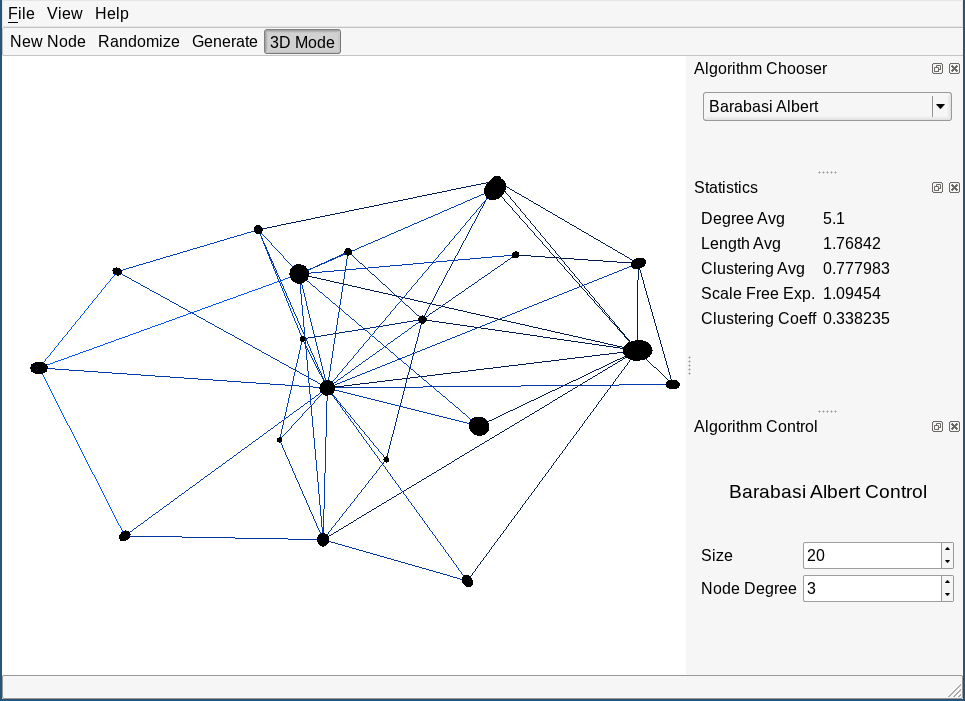
\includegraphics[width=1\textwidth]{screenshot-linux.png}
  Visigoth on Linux, 3D mode

  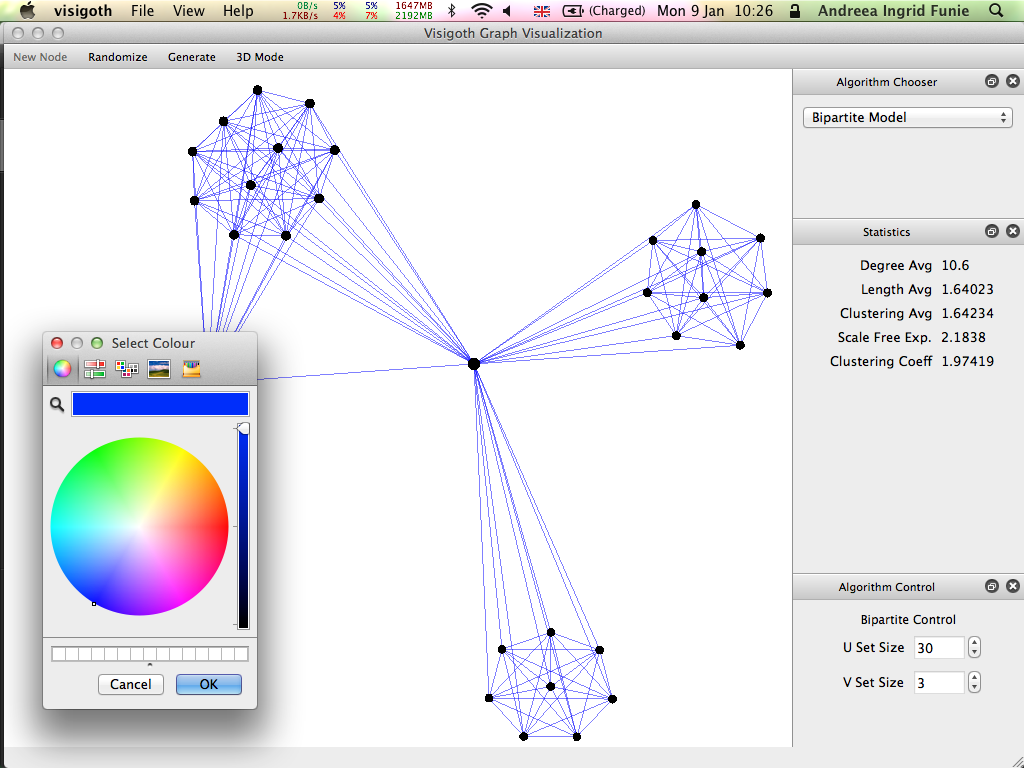
\includegraphics[width=1\textwidth]{screenshot-mac.png}
  Visigoth on Mac OS X, showing the ``Edge color'' dialog

  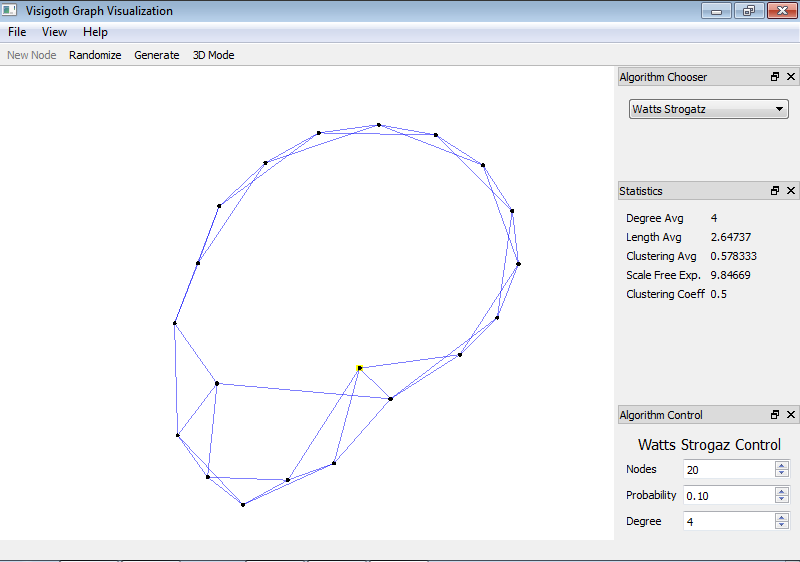
\includegraphics[width=1\textwidth]{screenshot-win.png}
  Visigoth on Windows
\end{center}

\section{Sample graphs}

Sample results of the 5 graph models employed by Visigoth, plus the Twitter
graph:

\begin{center}
  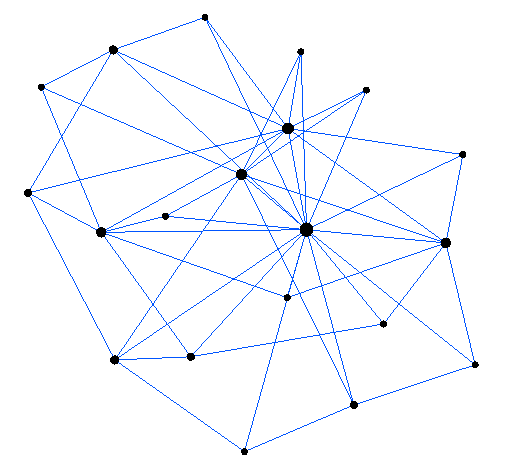
\includegraphics[width=0.5\textwidth]{barabasi.png}\\
  Barab\'{a}si-Albert

  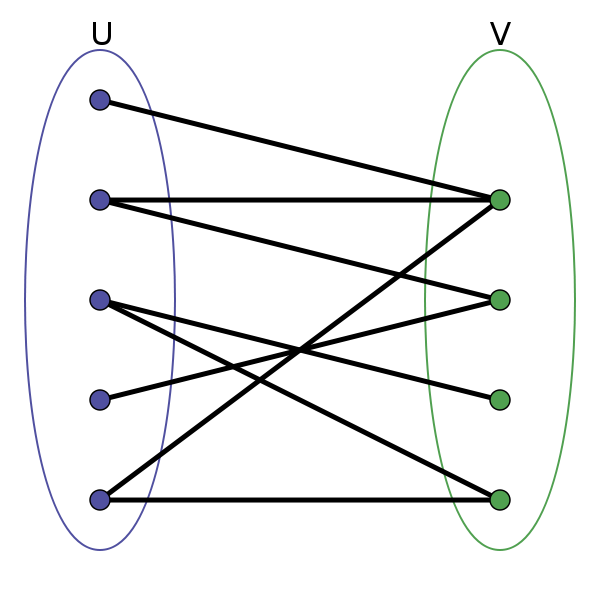
\includegraphics[width=0.5\textwidth]{bipartite.png}\\
  Bipartite

  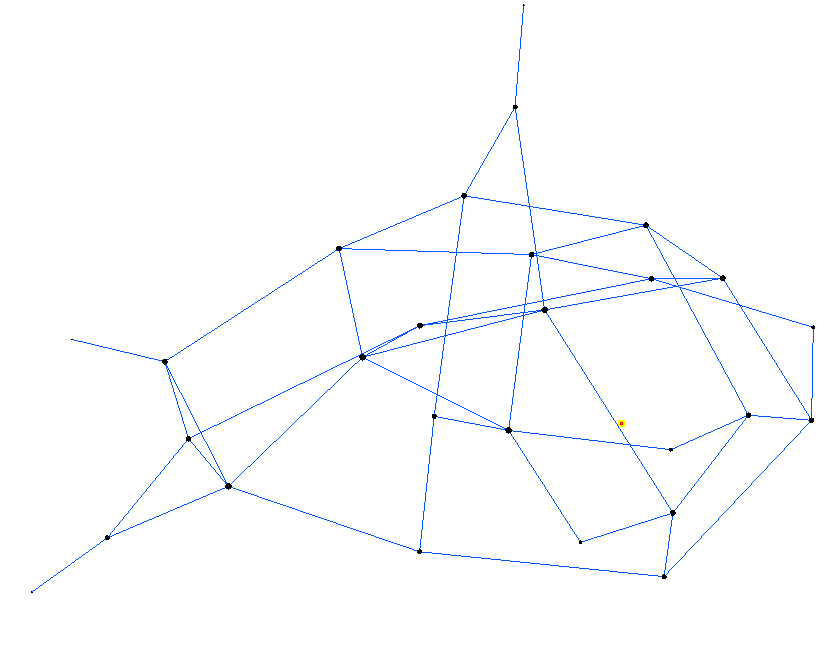
\includegraphics[width=0.5\textwidth]{erdos.png}\\
  Erd\H{o}s-R\'{e}nyi

  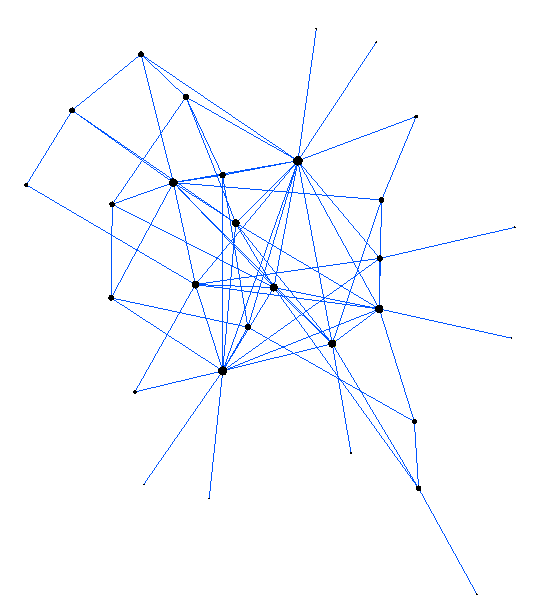
\includegraphics[width=0.5\textwidth]{preferential.png}\\
  Preferential attachment

  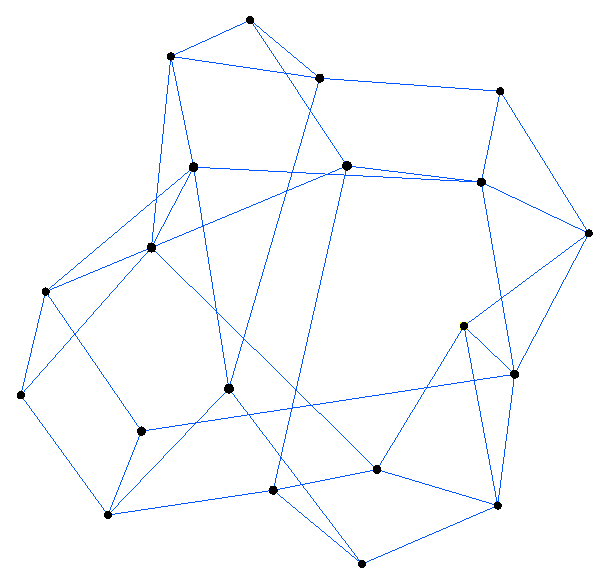
\includegraphics[width=0.5\textwidth]{watts.png}\\
  Watts-Strogatz

  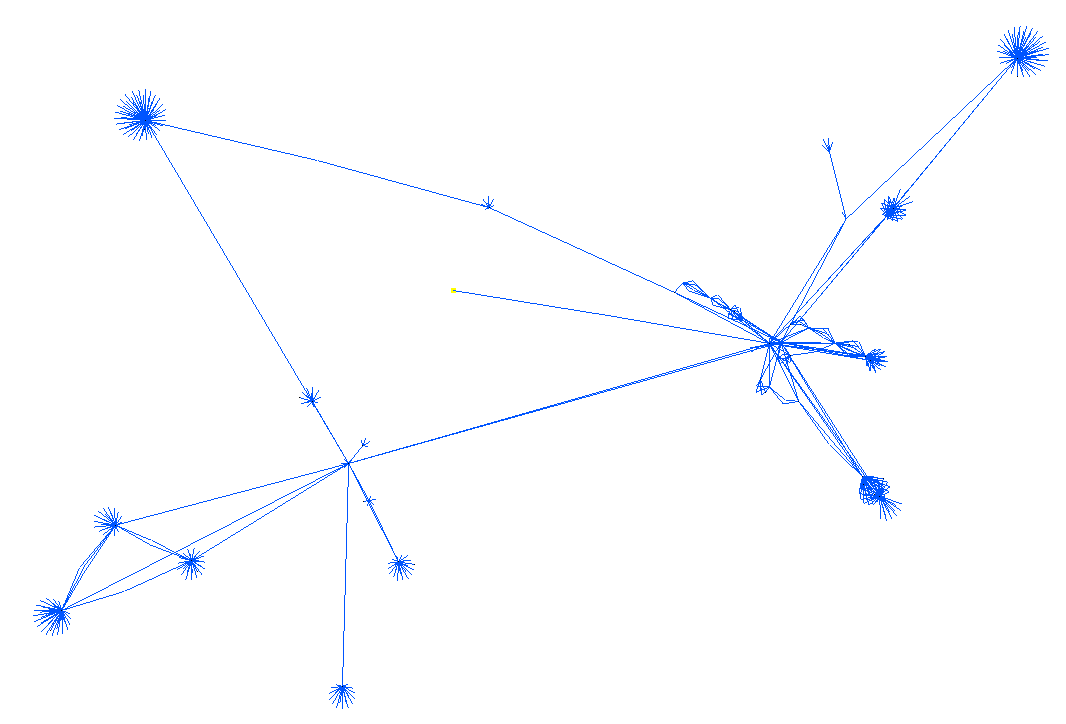
\includegraphics[width=0.5\textwidth]{twitter.png}\\
  Twitter
\end{center}

\addcontentsline{toc}{section}{References}
\begin{thebibliography}{9}

\bibitem{hamm10}
  David A. Hammond,
  \emph{Altruism in Small World Models}.
  Imperial College London,
  2010.

\bibitem{oconn11}
  Luke M. O'Connor,
  \emph{Algorithms for Constructing Realistic Networks}.
  Imperial College London,
  2011.

\bibitem{fade}
  Aaron Quigley and Peter Eades,
  \emph{FADE: Graph drawing, clustering and visual abstraction}.
  Department of Computer Science and Software Engineering,
  Univ. of  Newcastle, Australia, 2000.

\bibitem{complexAdapt}
  Claudius Gros,
  \emph{Complex and Adaptive Dynamical Systems}.
  Springer,
  2008.

\bibitem{complexNets}
  Wikipedia contributors,
  \emph{Complex network}.
  Wikipedia, The Free Encyclopedia, 1 Jan. 2012.

\bibitem{swphen}
  Wikipedia contributors,
  \emph{Small world experiment}.
  Wikipedia, The Free Encyclopedia, 28 Dec. 2011.

\bibitem{smnet}
  Wikipedia contributors,
  \emph{Small-world network}.
  Wikipedia, The Free Encyclopedia, 5 Jan. 2012.

\end{thebibliography}

\end{document}
